\documentclass[12pt]{report}
\usepackage{amsmath}
\usepackage{graphicx}
\usepackage[colorlinks=true, linkcolor=black, citecolor=black, filecolor=black, urlcolor=black]{hyperref}
\usepackage{lipsum}
\usepackage{pdfpages}
\usepackage{titlesec}
\usepackage{pdfpages}
\usepackage{geometry}
\usepackage{float}
\usepackage{hyperref}
\usepackage[utf8]{inputenc}
\title{Heat Production Management Project for Semester Project 2}
\author{Kacper Grzyb \and Sebestyen Deak \and Ignad Bozhinov \and Leonardo Gianola \and Levente Sohar}
\date{03-06-2024}

% Define a command to convert number section counting to alphabetical section counting
\makeatletter
\newcommand{\alphsection}{\@alph\c@section}
\makeatother

% Redefine the sectioning commands
\renewcommand{\thesection}{\thechapter\alphsection}
\titleformat{\section}
  {\normalfont\Large\bfseries}{\thesection}{1em}{}

\begin{document}
\begin{titlepage}
  \centering
  \vspace*{1cm}
  
  \Huge
  \textbf{Syddansk Universitet}
  
  \vspace{2cm}
  
  \Huge
  \textbf{Project Report}
  
  \vfill
  
  \large
  Faculty of Engineering.\\
  BSc in Software Engineering\\
  Supervisor: Sadok Ben Yahia\\
  Project period: 2024.02.01 -- 2024.06.03.
  
  \vfill
  \begin{flushleft}  
    Group 11\\
    Participants: \\
  \end{flushleft}

    \hfill \small{\textbf{Kacper Grzyb} (kagrz23@student.sdu.dk)} \\
    \hfill \small{\textbf{Leonardo Gianola} (legia23@student.sdu.dk)} \\
    \hfill \small{\textbf{Levente Sohár} (lesoh23@student.sdu.dk)} \\
    \hfill \small{\textbf{Ignat Bozhinov} (igboz23@student.sdu.dk)} \\
    \hfill \small{\textbf{Sebestyén Deák} (sedea23@student.sdu.dk)} \\

\end{titlepage}

\tableofcontents

% Chapter 1
\chapter{Introduction}

\section*{Abstract}
This project report aims at designing and developing a web-application with a heat production optimization system in the imaginary city of Heatington. The objective is to minimize costs and maximize profits from electricity production while ensuring consistent heat delivery all year round. The system includes multiple modules, some of the key ones being: an Asset Manager, Source Data Manager, Result Data Manager, an Optimizer, and a Data Visualization module. This project addresses the transition from manual to optimized scheduling of heat production, leveraging advanced data management and optimization techniques.

\section{Background}
Heatington's district heating network is an essential aspect of urban distribution and supplies heat to a large number of structures through a system of pipelines and production units. The Combined Heat and Power (CHP) network incorporates both conventional heat-only boilers and CHP units that produce both heat and power. Originally, the scheduling of these heat production units has been done in a manual manner, compromising efficiency and incurring high costs. New energy market conditions, with their constant calls for economic efficiency in the energy production process, demand a more complex and automated approach to the scheduling of heat production.

District heating systems centralize the production of heat and distribute it through hot water to different buildings in the city. The heat from the hot water is used for both heating the building and preparing hot water for the occupants. After releasing its heat, the cooled water is recirculated back to the plant where it is reheated. This cycle ensures a constant provision of heat, although controlling it is always a challenge given the unpredictable nature of heat demand at different times and seasons.

\section{Project Brief}
Developing an optimization system that schedules heat production for Heatington's district heating network at the lowest possible cost while maximizing profit from electricity production is the main goal of this semester-long project. The system is designed to handle data from different production units, factoring in production costs, electricity prices, and heat demand to generate optimal schedules that ensure operational efficiency and financial profitability.

The system comprises several key modules:

\begin{itemize}
    \item \textbf{Asset Manager (AM)}: Captures non-operational data of the heating grid and production units, including operational conditions, production rates, cost data, and CO2 emission rates. It ensures that the most up-to-date information required for optimization processes and other system elements is available.
    \item \textbf{Source Data Manager (SDM)}: Processes dynamic data such as heat demand and electricity prices in the form of time series, as the heating grid requirements often change over time. The SDM aids the optimization process by providing the temporal context for scheduling decisions.
    \item \textbf{Result Data Manager (RDM)}: Stores optimized scheduling results and performance data for each production unit. This module retains copies of all results for validation, reporting, or further analysis.
    \item \textbf{Optimizer (OPT)}: The core component responsible for calculating optimal heat production schedules. It considers all available production units, their costs, and electricity market dynamics to generate schedules that secure heat availability while minimizing costs. The Optimizer will be implemented in two scenarios to progressively incorporate complexity, starting with basic heat-only units and extending to include electricity-producing and consuming units.
    \item \textbf{Data Visualization (DV)}: Provides a graphical interface to review the heating grid format, production facilities, and optimization outcomes. This module enhances system usability by allowing stakeholders to easily understand metrics, time series, and overall system performance through graphical representations.
\end{itemize}

This project enables Heatington’s district to efficiently and automatically generate the best schedule, ensuring adequate, cost-effective, and reliable heat delivery to its residents.

% Chapter 2
\chapter{Release Planning}
This chapter contains the release planning as we wrote it before the first sprint. As the project matured we made more accurate representations, which are included in the Sprint Materials chapter.
\section*{User Stories}
\subsection*{Heating System Manager}
As a Heating System Manager, I want to visualize real-time heat production data (produced heat, produced/consumed electricity, production costs, consumption of primary energy and produced amount of CO2) through a user-friendly dashboard that allows me to choose the period I want that helps me make informed decisions, optimize heat production and minimize costs. \\
HIGH Priority, 13 User Points\\
Connected Requirements: Result Data Manager, Optimizer
\subsection*{Data Administrator}
As a Data Administrator for the heat production optimization application, I need to effectively import data to ensure optimal performance and efficiency of the heat production system. \\
HIGH Priority, 8 User Points\\
Connected Requirements: Source Data Manager, Asset Manager
\subsection*{Financial Analyst}
As Financial Analyst I want to look at previous month's data and look for improvement. I must know when it's the best time to buy electricity, and when to sell it. I need to know which machines are the most efficient, and whether it's the best for the company to keep the already used machines, or to change some of them. For this I need to see the operation costs and a few graphs. \\
MEDIUM Priority, 13 User Points\\
Connected Requirements: Result Data Manager, Data Visualization
\subsection*{Sustainability Officer}
As a Sustainability Officer I want to promote sustainable energy practices. With background in environmental engineering and deep commitment to combating climate change I want an application where I can easily visualize the emission and the potential improvements I can make.\\
LOW Priority, 5 User Points\\
Connected Requirements: Result Data Manager, Data Visualization
\clearpage

\section*{Definition of Done}

\begin{itemize}
  \item Result Data Manager component finished
  \item Asset Manager component finished
  \item Source Data Manager component finished
  \item Optimizer component finished
  \item Continuous Integration implemented with at least 60 \% code coverage
  \item UI Elements are functional and responsive across all devices
  \item UX reviewed and tested by external users
  \item Reviewed by Product Owner
  \item Group Supervisor has reviewed and approved the features
  \item All known bugs and issues are resolved and documented
  \item Third party libraries are properly licensed
  \item Product increment has been built into release mode and tested by the team
  \item All release documentation has been written and reviewed by group supervisor
  \item Scenario 1 and 2 are Implemented
\end{itemize}


% Chapter 3
\chapter{Sprint Materials}
\label{sec:sprints}
In this chapter all the materials from the sprints can be found.




\section{Sprint 1}
%Review
\subsection*{Sprint Review}
\textbf{Project:} Semester Project Group 11 \\
\textbf{Sprint Duration:} March 5 - March 19, 2024 \\
\textbf{Team Members:} Kacper Grzyb, Sebestyen Deak, Ignat Bozhinov, Leonardo Gianola, Levente Sohar \\
\textbf{Stakeholders:} Sadok Ben Yahia

\subsection*{1. Sprint Goals and Outcomes}

\begin{itemize}
    \item \textbf{Goal 1:} Move epic and user stories into Jira\\
    \textbf{Status:} Completed. All the epics and user stories are in Jira now.
    \item \textbf{Goal 2:} Divide Roles\\
    \textbf{Status:} Completed. Product Owner and Scrum Master Roles have been given.
    \item \textbf{Goal 3:} Create .gitignore file\\
    \textbf{Status:} Completed. Created .gitignore file.
    \item \textbf{Goal 4:} Break down User Stories into requirements with MoSCoW\\
    \textbf{Status:} Completed. All the different User Stories have a Must Do (-M), Should Do (-S), Can Do (-C), Would Not Do (-W).
    \item \textbf{Goal 5:} Rewrite tasks into User Stories\\
    \textbf{Status:} Completed.
    \item \textbf{Goal 6:} Add User Points to User Stories\\
    \textbf{Status:} Completed. Every User Story has been rated in story points.
    \item \textbf{Goal 7:} Gantt Chart\\
    \textbf{Status:} Completed. Every Task has been estimated, and a Gantt Chart has been made according to this and our timeframe.
    \item \textbf{Goal 8:} Create Sprint Review\\
    \textbf{Status:} Completed.
\end{itemize}

\subsection*{2. Completed Work}
Transitioning our project management to Jira, we've streamlined our workflow and enhanced visibility into our tasks and progress. Recognizing the importance of role clarity in optimizing team performance, we successfully delineated roles and responsibilities. Implementing best practices in version control, we established a .gitignore file. Employing the MoSCoW method to prioritize requirements, we gained clarity on project scope and stakeholder expectations. Restructuring our tasks into user stories, we've shifted our focus from implementation details to user-centric outcomes, fostering a deeper understanding of user needs and motivations. Introducing user points to our user stories allowed us to quantify complexity and effort more accurately, facilitating resource allocation and sprint planning. Creating a Gantt chart provided us with a visual roadmap for project execution, enabling us to sequence tasks, allocate resources, and identify dependencies more effectively. Instituting sprint reviews has fostered transparency, accountability, and continuous improvement within our agile framework.
\subsection*{3. Unfinished Work}
Everything we set out to do during this sprint we have accomplished.
\subsection*{4. Quality and Technical Issues}
We haven't started coding yet, and only used already established software for our work, therefore we didn't have any technical issues.
\subsection*{5. Team Dynamics and Collaboration}
Work has been mostly divided equally, with everyone doing their part. Communication was clear and to the point.
\subsection*{6. Processes and Tools}
Jira helps keep track of the backlog and manage the sprint. For making the Gantt Chart, Canva was used, which helped speed up the process.
\subsection*{7. Stakeholder Feedback}
When talking with our supervisor Sadok, he approved of the direction we were heading this sprint, emphasizing making Dashboards.
\subsection*{8. Obstacles and Impediments}
We have been able to complete all the goals without any obstacles or impediments.
\subsection*{9. Successes and Wins}
The biggest win for the team was finishing all of our goals in time.
\subsection*{10. Action Items for Improvement}
Breaking the requirement into small tasks that can be worked on independently, therefore not everything has to be done in the one meeting we weekly.

\hfill 16/03/2024


\begin{figure}[H]
  \centering
  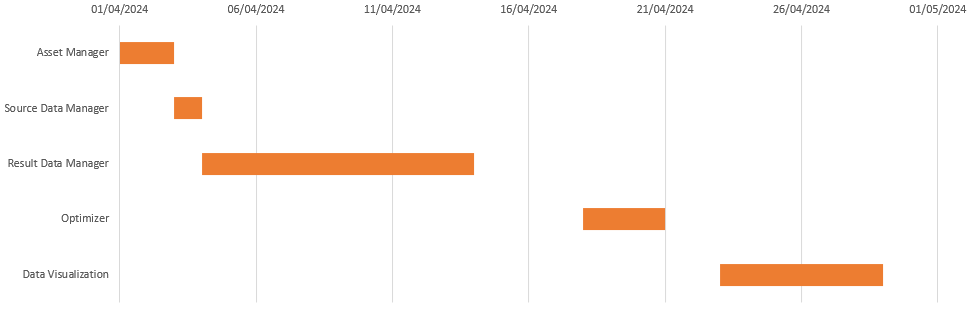
\includegraphics[width=1\textwidth]{Resources/1-Sprint/Gantt-Chart-Optimal.png}
  \caption{Optimal Gantt Chart}
  \label{fig:OptGanttChart}
\end{figure}

\begin{figure}[H]
  \centering
  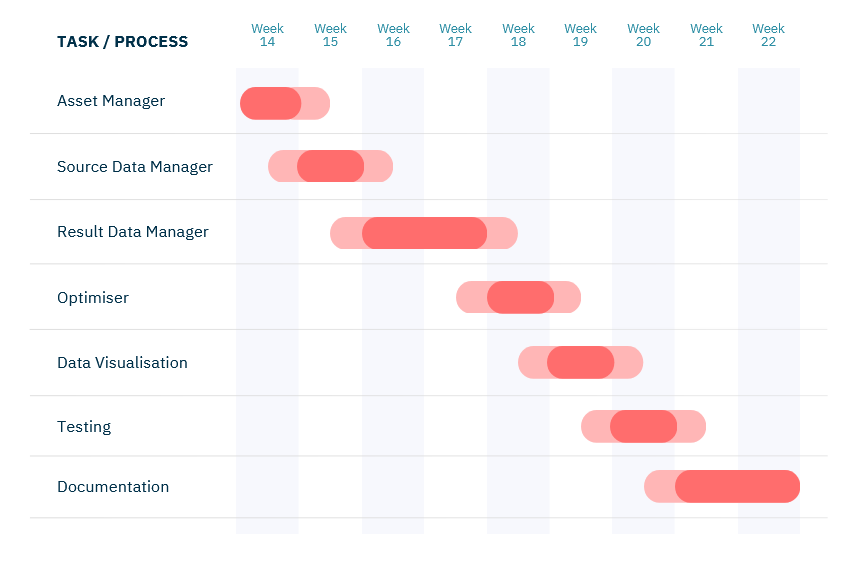
\includegraphics[width=1\textwidth]{Resources/1-Sprint/Gantt-Chart-Realistic.png}
  \caption{Realistic Gantt Chart}
  \label{fig:RealGanttChart}
\end{figure}
\clearpage





\section{Sprint 2}
%Planning
\subsection*{Planning}
\begin{figure}[H]
  \centering
  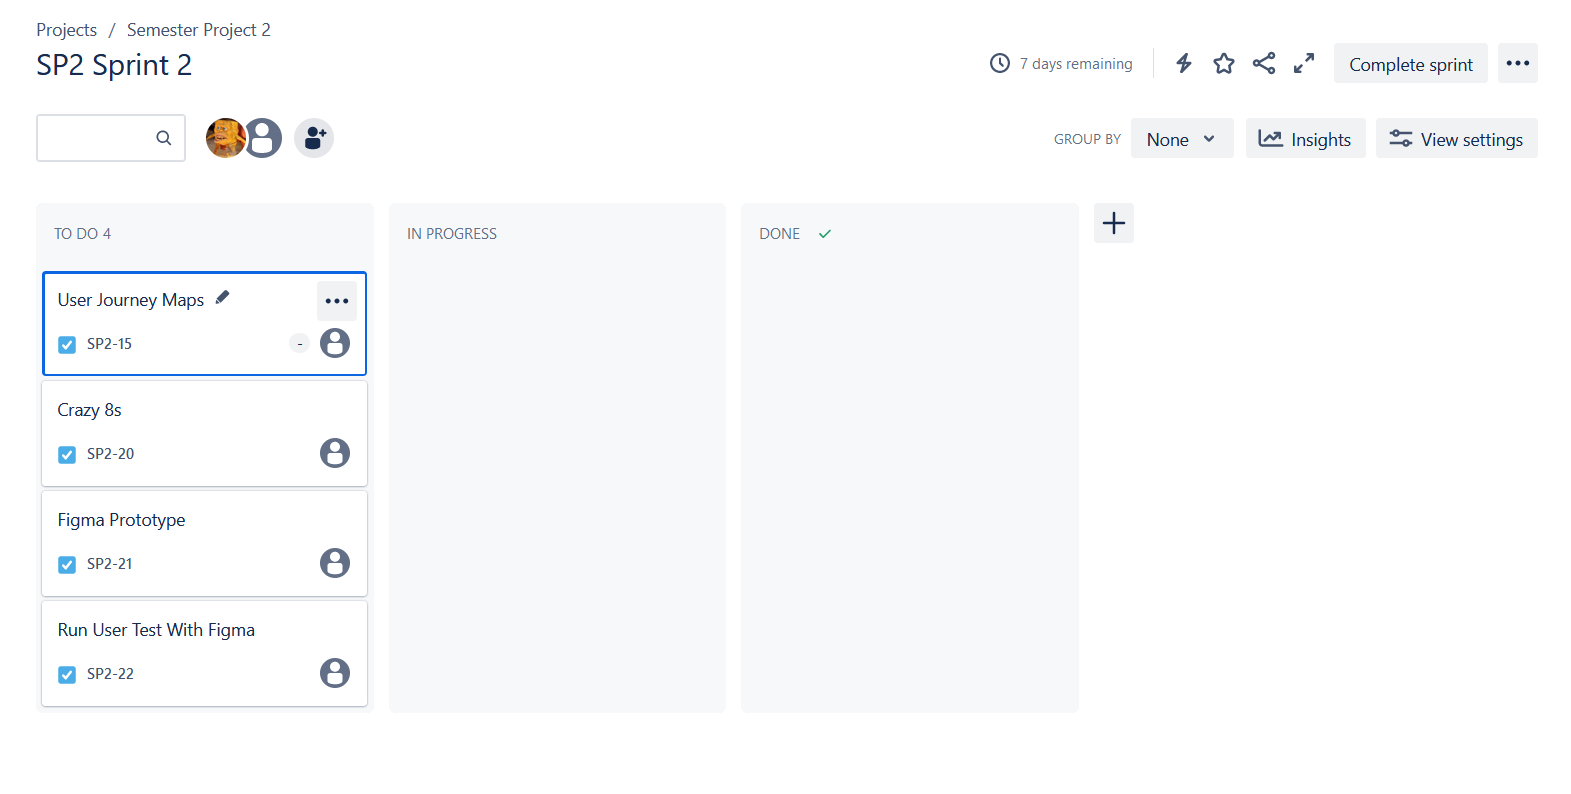
\includegraphics[width=1\textwidth]{Resources/2-Sprint/Planning/Sprint2_Planning_Package.png}
  \caption{Sprint 2 Planning Package}
  \label{fig:S2Planning}
\end{figure}

%Daily Scrum
\subsection*{Daily Scrum 02/04/2024}

\begin{itemize}
    \item The team completed 2 out of 4 issues.
    \item 2 issues are currently in progress, one of which is very close to being finished and the other one is expected to be finished by the end of the week.
\end{itemize}

\subsection*{Roadblocks}
\begin{itemize}
    \item The team faced a few conflicting ideas and a wrong understanding of how the Result Data Manager and Asset Manager components are supposed to look like. They were solved through an online Discord meeting.
    \item Some team members are still on holidays, which makes organising work a bit harder.
\end{itemize}

\subsection*{Plans for the rest of the Sprint}
\begin{itemize}
    \item Polish the Figma prototype made.
    \item Get feedback on the Figma prototype.
    \item Begin discussion about starting the development phase.
\end{itemize}

\subsection*{Metrics and Progress}
The team has attached screenshots of the current state of the sprint backlog and the sprint status report to give information about how much work has been done and how much work still needs to be done.

\begin{figure}[H]
  \centering
  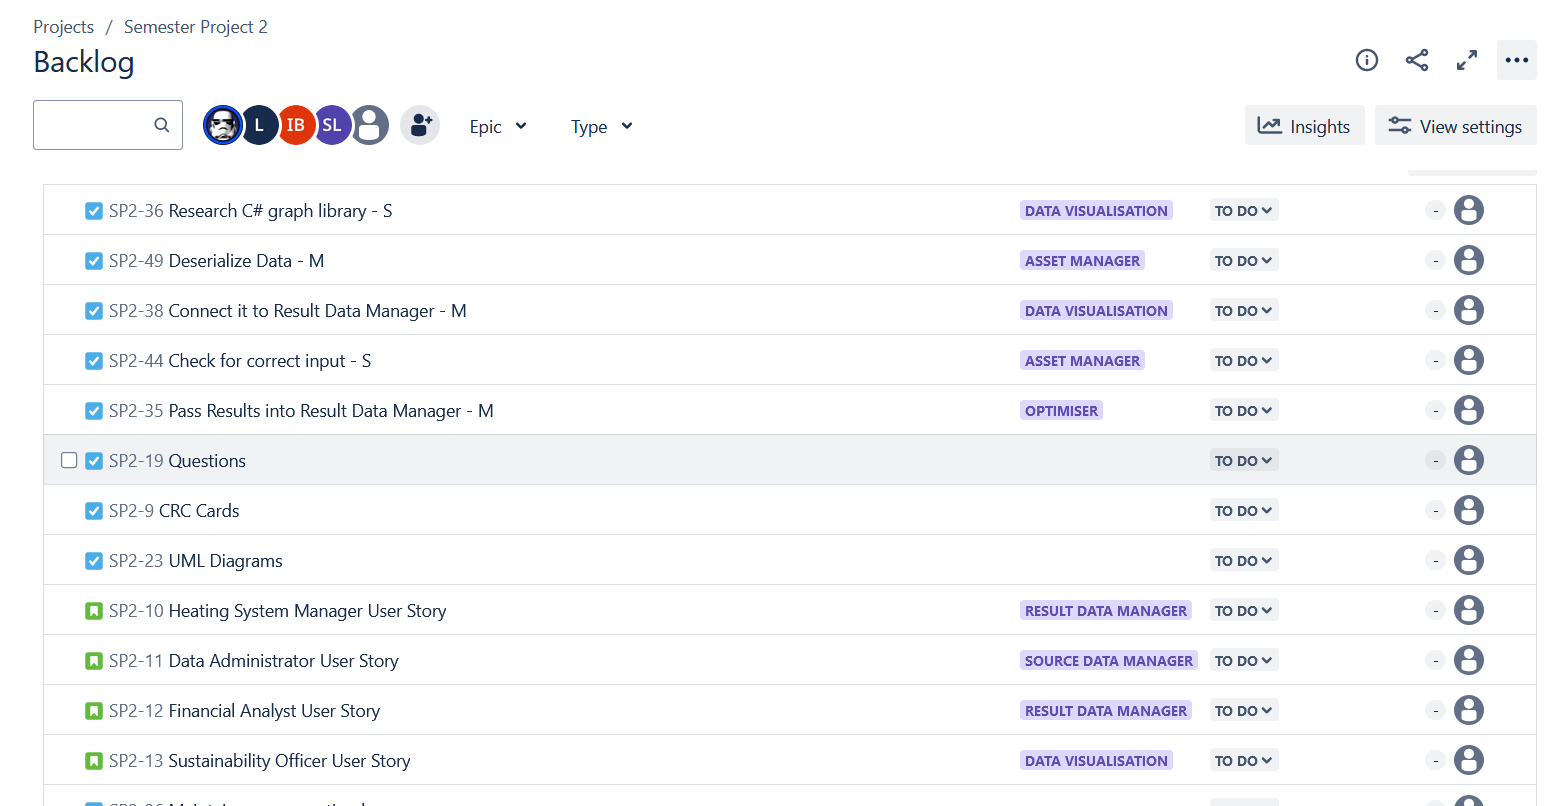
\includegraphics[width=1\textwidth]{Resources/2-Sprint/Daily-Scrum/backlog1.png}
  \caption{Daily Scrum Backlog 1}
  \label{fig:S2Scrum1-image}
\end{figure}

\begin{figure}[H]
  \centering
  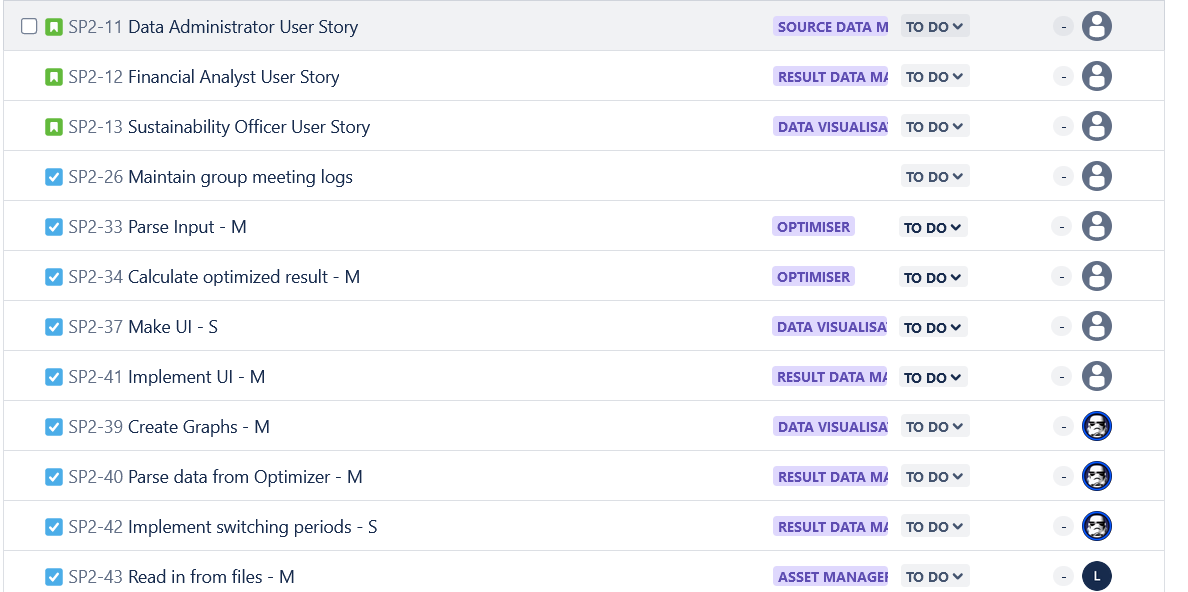
\includegraphics[width=1\textwidth]{Resources/2-Sprint/Daily-Scrum/backlog2.png}
  \caption{Daily Scrum Backlog 2}
  \label{fig:S2Scrum2-image}
\end{figure}

\begin{figure}[H]
  \centering
  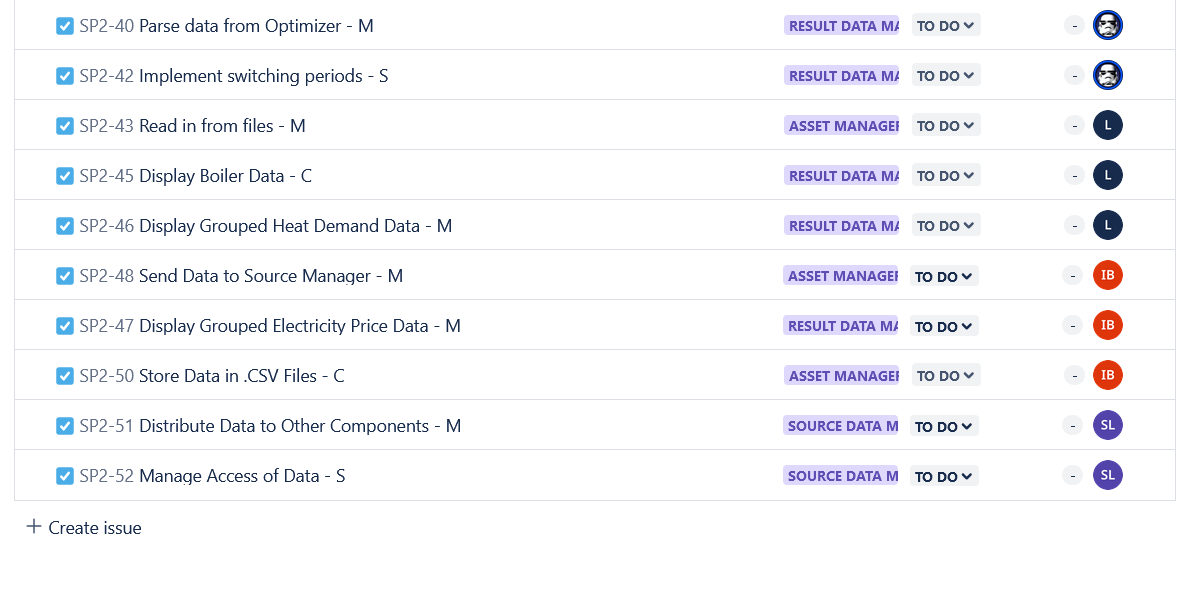
\includegraphics[width=1\textwidth]{Resources/2-Sprint/Daily-Scrum/backlog3.png}
  \caption{Daily Scrum Backlog 3}
  \label{fig:S2Scrum3-image}
\end{figure}

%Retrospective

\subsection*{Sprint Review}

\subsection*{What went well}
\begin{itemize}
    \item Remote meeting to re-align on the project direction
    \item All sprint tasks done despite remote work due to the Easter holidays
    \item Remote communication
    \item Willingness to pivot, make changes to the project
\end{itemize}

\subsection*{What to improve}
\begin{itemize}
    \item Spend more time on understanding the project requirements -- the team had a wrong idea of what the Result Data Manager, Asset Manager and Source Data Manager should consist of which created a setback and meant some of the plans for the project need to be remade, such as the tasks on Jira
    \item Pay attention to time zones when doing remote work -- the time zone difference created a minor issue during one of the team's remote meetings
    \item Plan out and divide work more carefully to avoid misunderstandings and vagueness
\end{itemize}

\subsection*{What the team aims to improve in the next Sprint}
\begin{itemize}
    \item Align the project with the requirements
    \item Remove vagueness from the project direction
    \item Remove vagueness from tasks for each team member
\end{itemize}
\clearpage




\section{Sprint 3}
%Planning
\subsection*{Planning}
The team's goal for this sprint is to be ready for the Midterm Evaluation that is to happen on
Wednesday the 17th of March. The team has planned out to work on the 3 required components:
Result Data Manager, Asset Manager and Source Data Manager. The components will be created in
Asp.Net using Razor Pages and only the boiler configuration for the first iteration will be supported
by the app created. The components will be developed throughout the week depending on the time
of each individual developer . Only one team member was missing during the Sprint 3 Planning
Meeting, and he will be informed of everything discussed through online matters. The only issue that
made the planning process harder was the Jira backlog being outdated due to the product vision
changes. This will be fixed in a future sprint.

\begin{figure}[H]
  \centering
  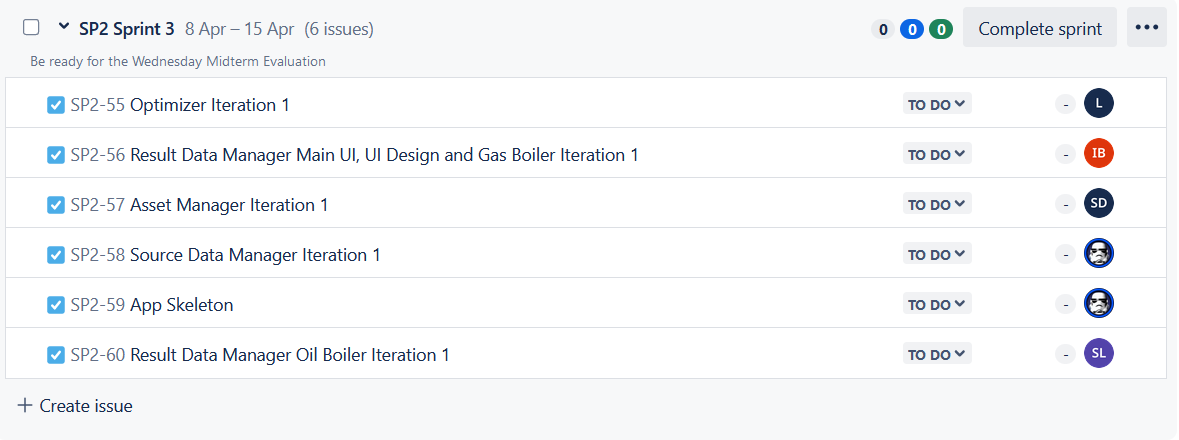
\includegraphics[width=1\textwidth]{Resources/3-Sprint/Planning/Sprint3Planning.png}
  \caption{Sprint 3 Planning}
  \label{fig:S3Planning-image}
\end{figure}
\clearpage

%Scrum
\subsection*{Daily Scrum 16/04/2024}
\subsection*{Team Update}
\begin{itemize}
    \item The team completed 6 out of 6 issues.
    \item The goal for the sprint of being ready for the first iteration presentation has been met.
\end{itemize}

\subsection*{Roadblocks}
\begin{itemize}
    \item Most of the development did not see any roadblocks due to deliberate planning done beforehand.
    \item Team members helped each other to make sure no one is stuck, and the tasks are finished on time.
\end{itemize}

\subsection*{Plans for the Next Sprint}
\begin{itemize}
    \item Fix bugs.
    \item Continue development.
\end{itemize}

\subsection*{Metrics and Progress}
The team has attached screenshots of the current state of the sprint backlog and the sprint status report to give information about how much work has been done and how much work still needs to be done.

\begin{figure}[H]
  \centering
  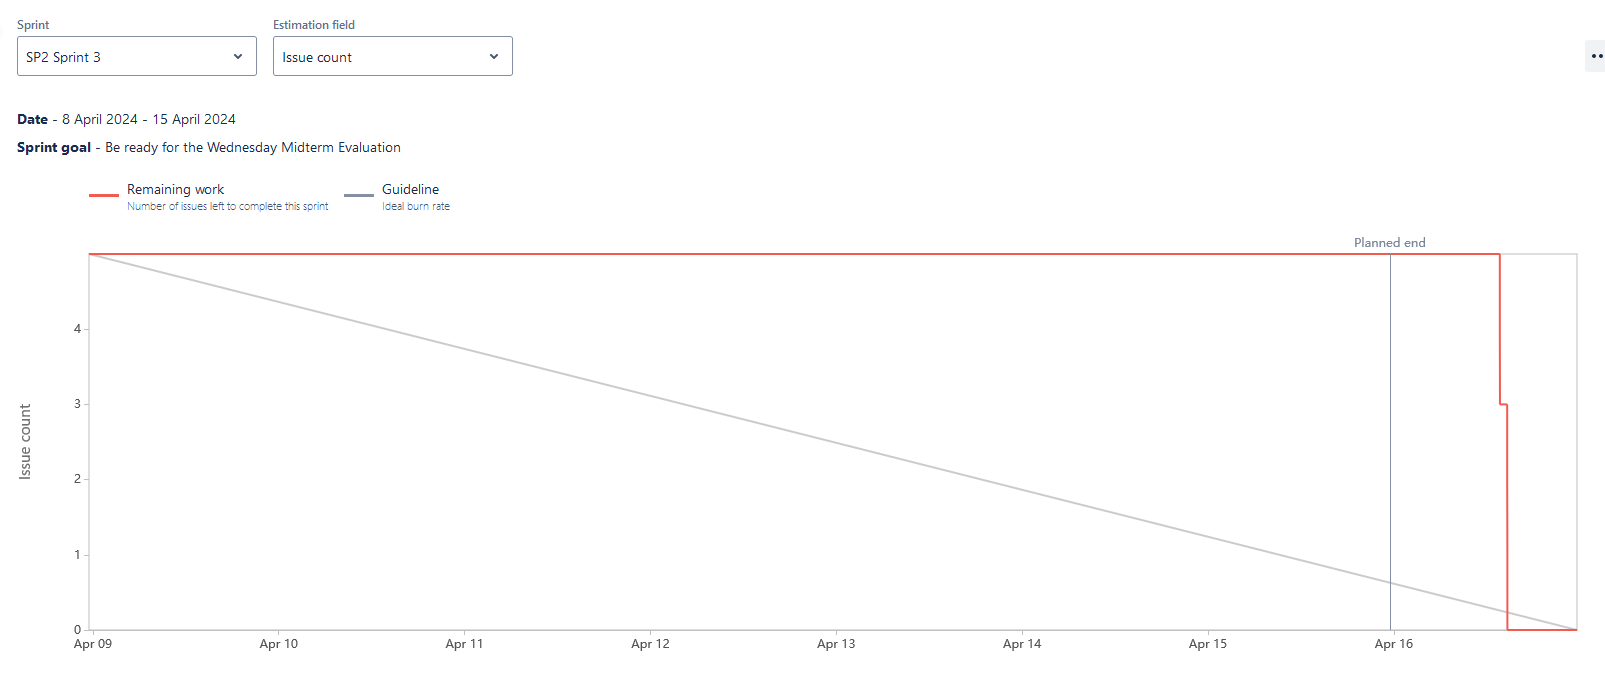
\includegraphics[width=1\textwidth]{Resources/3-Sprint/Daily-Scrum/burndownchart_sprint3.png}
  \caption{Daily Scrum Burndown Chart}
  \label{fig:S3Scrum2-image}
\end{figure}

\begin{figure}[H]
  \centering
  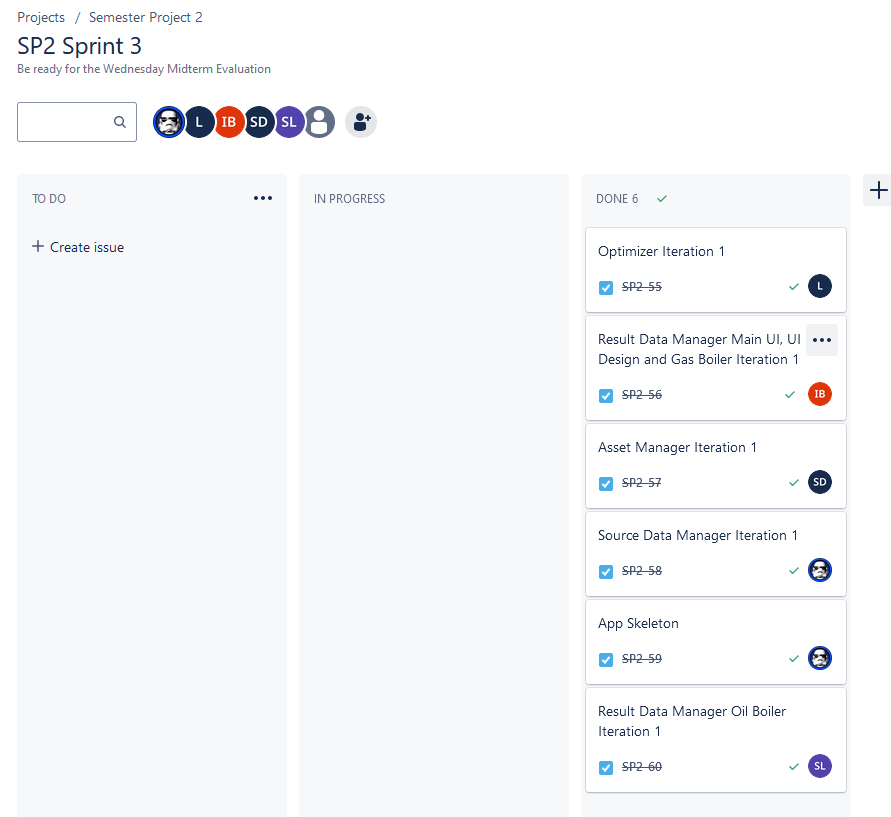
\includegraphics[width=1\textwidth]{Resources/3-Sprint/Daily-Scrum/backlog_sprint3.png}
  \caption{Daily Scrum Backlog}
  \label{fig:S3Scrum1-image}
\end{figure}

\clearpage

%Review

\subsection*{Sprint Review}
\textbf{Project:} Semester Project Group 11 \\
\textbf{Sprint Duration:} April 9 - April 23, 2024 \\
\textbf{Team Members:} Kacper Grzyb, Sebestyen Deak, Ignat Bozhinov, Leonardo Gianola, Levente Sohar \\
\textbf{Stakeholders:} Sadok Ben Yahia

\subsection*{1. Sprint Goals and Outcomes}
During this sprint, we aimed to iterate our plans for the optimizer program and make a working prototype for the presentation.

\begin{itemize}
    \item \textbf{Goal 1:} Optimizer iteration 1\\
    \textbf{Status:} Completed. The optimizer (for now) looks at the heat demands and if it's below the gas boiler capacity, it only uses that. If exceeded, the other boiler turns on.
    \item \textbf{Goal 2:} UI, UI Design and Gas Boiler Iteration 1\\
    \textbf{Status:} Completed. The app skeleton has been created using Bootstrap for better UX.
    \item \textbf{Goal 3:} Asset Manager Iteration 1\\
    \textbf{Status:} Completed. Created classes for all the boilers, both for iteration 1 and 2.
    \item \textbf{Goal 4:} Source Data Manager Iteration 1\\
    \textbf{Status:} Completed - with minor issue. The Source Data Manager reads in the data from CSV files and creates objects from it. The only issue we have with it is that since Apple's MacOS uses a different DateTime format than Windows, it throws an exception for some of the dates.
    \item \textbf{Goal 5:} Result Data Manager Oil Boiler Iteration 1\\
    \textbf{Status:} Completed.
\end{itemize}

\subsection*{2. Completed Work}
We had the midterm presentation during this sprint, so our main focus was on getting the program in a state that can be presented and making the presentation. We focused on not just making the program work, but also making it easily expandable, therefore we have less work to do in the second iteration. For the visual UI, we used Razor pages, and in that Bootstrap. We made all the components work almost flawlessly, and the end result visually remained close to our Figma prototype.
\subsection*{3. Unfinished Work}
Everything we set out to do during this sprint we have accomplished.
\subsection*{4. Quality and Technical Issues}
There remained to be a bug, where Mac devices aren't able to read in all the data from the CSV file, since the OS expects the months to be where the days are in the source data. So after the day exceeds the 13th day, it throws an exception.
\subsection*{5. Team Dynamics and Collaboration}
Work has been mostly divided equally, with everyone doing their part. Communication was clear and to the point. We had weekly meetings for scrum.
\subsection*{6. Processes and Tools}
Jira helps keep track of the backlog and manage the sprint. Razor pages and Bootstrap have been used for UI. We sometimes looked back at our Figma prototype for reference.
\subsection*{7. Stakeholder Feedback}
After our midterm presentation, we got feedback from 2 supervisors, both were supportive of our development methods and the state of the program. The only criticism we got was regarding our presentation style, and we will try to keep that in mind for the next time.
\subsection*{8. Obstacles and Impediments}
We have been able to complete all the goals without any obstacles or impediments.
\subsection*{9. Successes and Wins}
The biggest win for the team was the feedback we got after the presentation both from the supervisors and the other students.
\subsection*{10. Action Items for Improvement}
Setting a hierarchy amongst tasks so no one has to wait for the other to finish.

\hfill 24/04/2024
\clearpage







\section{Sprint 4}
%Planning
\subsection*{Planning}
The team's aim for this sprint is to try and make the final product, since we only have about 4-5 weeks before having to present it in front of the other students and teachers. This means updating the optimizer, and the UI. We also plan on adding graphs which show the given data, in various configurations. We also plan to fix the bug with the Source Data Manager. Two team members were missing during the Sprint 4 Planning Meeting, but we talked about our goals previously and they will be informed of everything discussed through online matters.

\begin{figure}[H]
  \centering
  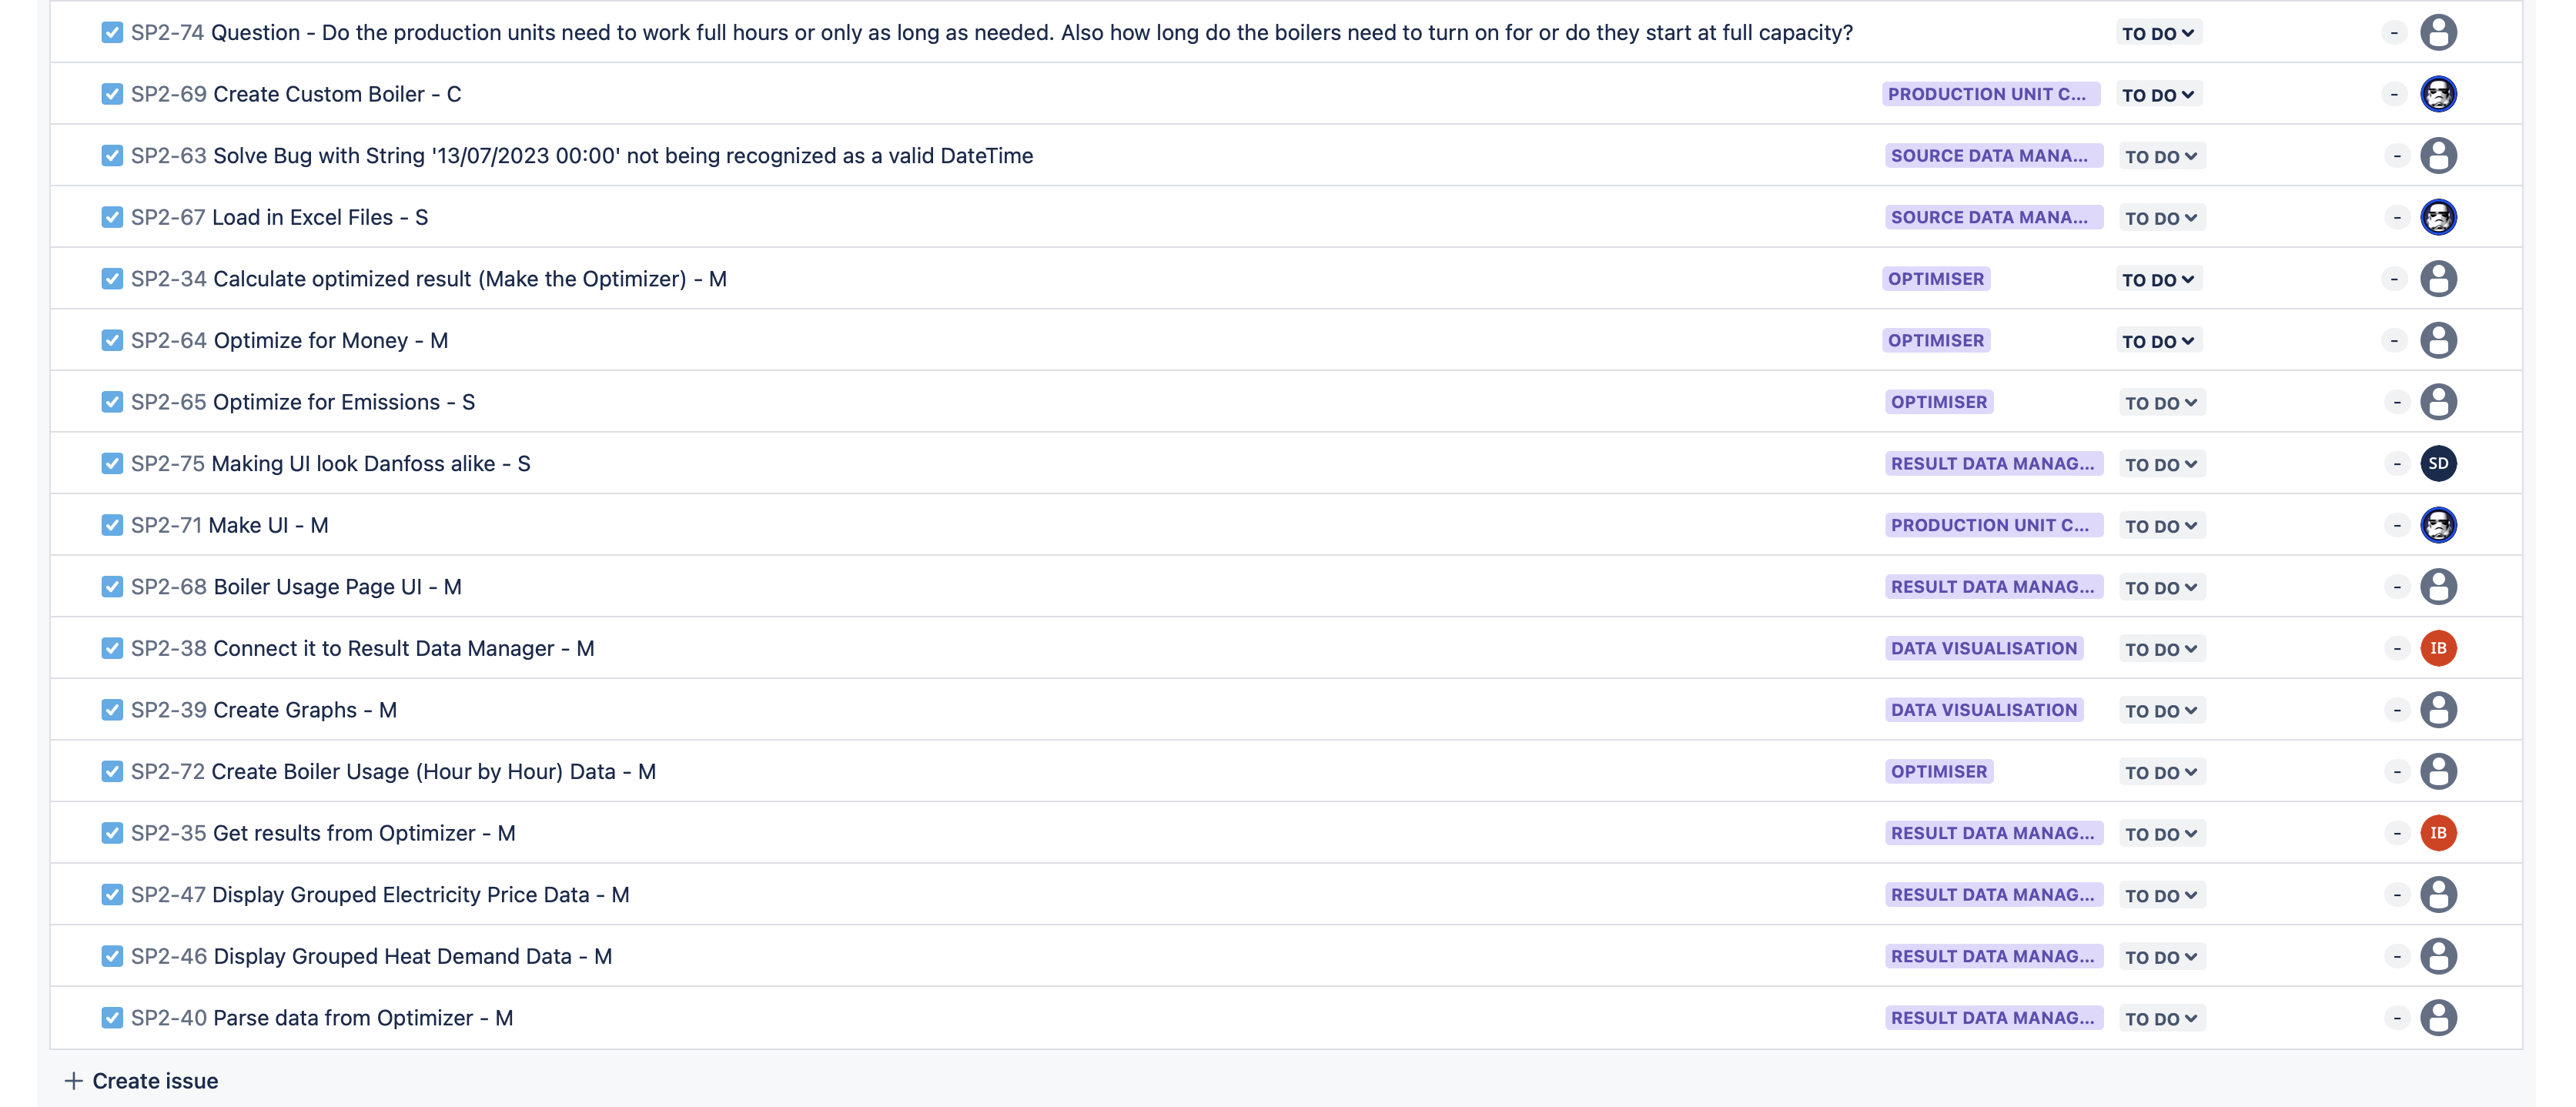
\includegraphics[width=1\textwidth]{Resources/4-Sprint/Planning/Jira.png}
  \caption{Planning Backlog}
  \label{fig:S4Planning-image}
\end{figure}
\clearpage

%Scrum

\subsection*{Daily Scrum 29/04/2024}
\subsection*{Team Update}
\begin{itemize}
    \item The team finished 7 issues and made major progress towards the biggest issue out of 24 issues in the current sprint.
    \item Kacper and Sebestyén will finish work on the optimizer and work on other tasks while Leonardo will continue to work on his neural network optimizer until the end of the sprint. Ignat and Levente are moving on to other tasks.
    \item The goal for the sprint is to complete as many issues as possible.
\end{itemize}

\subsection*{Roadblocks}
\begin{itemize}
    \item The team needed to realign on the approach for the implementation of the optimizer, change the implementation of some of the data structures and get everyone on the same page in the code structure.
    \item Every roadblock was talked about and resolved on this Monday’s meeting.
\end{itemize}

\subsection*{Plans for the Next Sprint}
\begin{itemize}
    \item Continue completing issues from the backlog, while focusing on the must-have features.
    \item Come up with a solution for having multiple optimizers and custom production units.
    \item Make sure all requested features are accounted for in the sprint backlog.
\end{itemize}

\subsection*{Metrics and Progress}
The team has attached screenshots of Jira for progress metrics.

\begin{figure}[H]
  \centering
  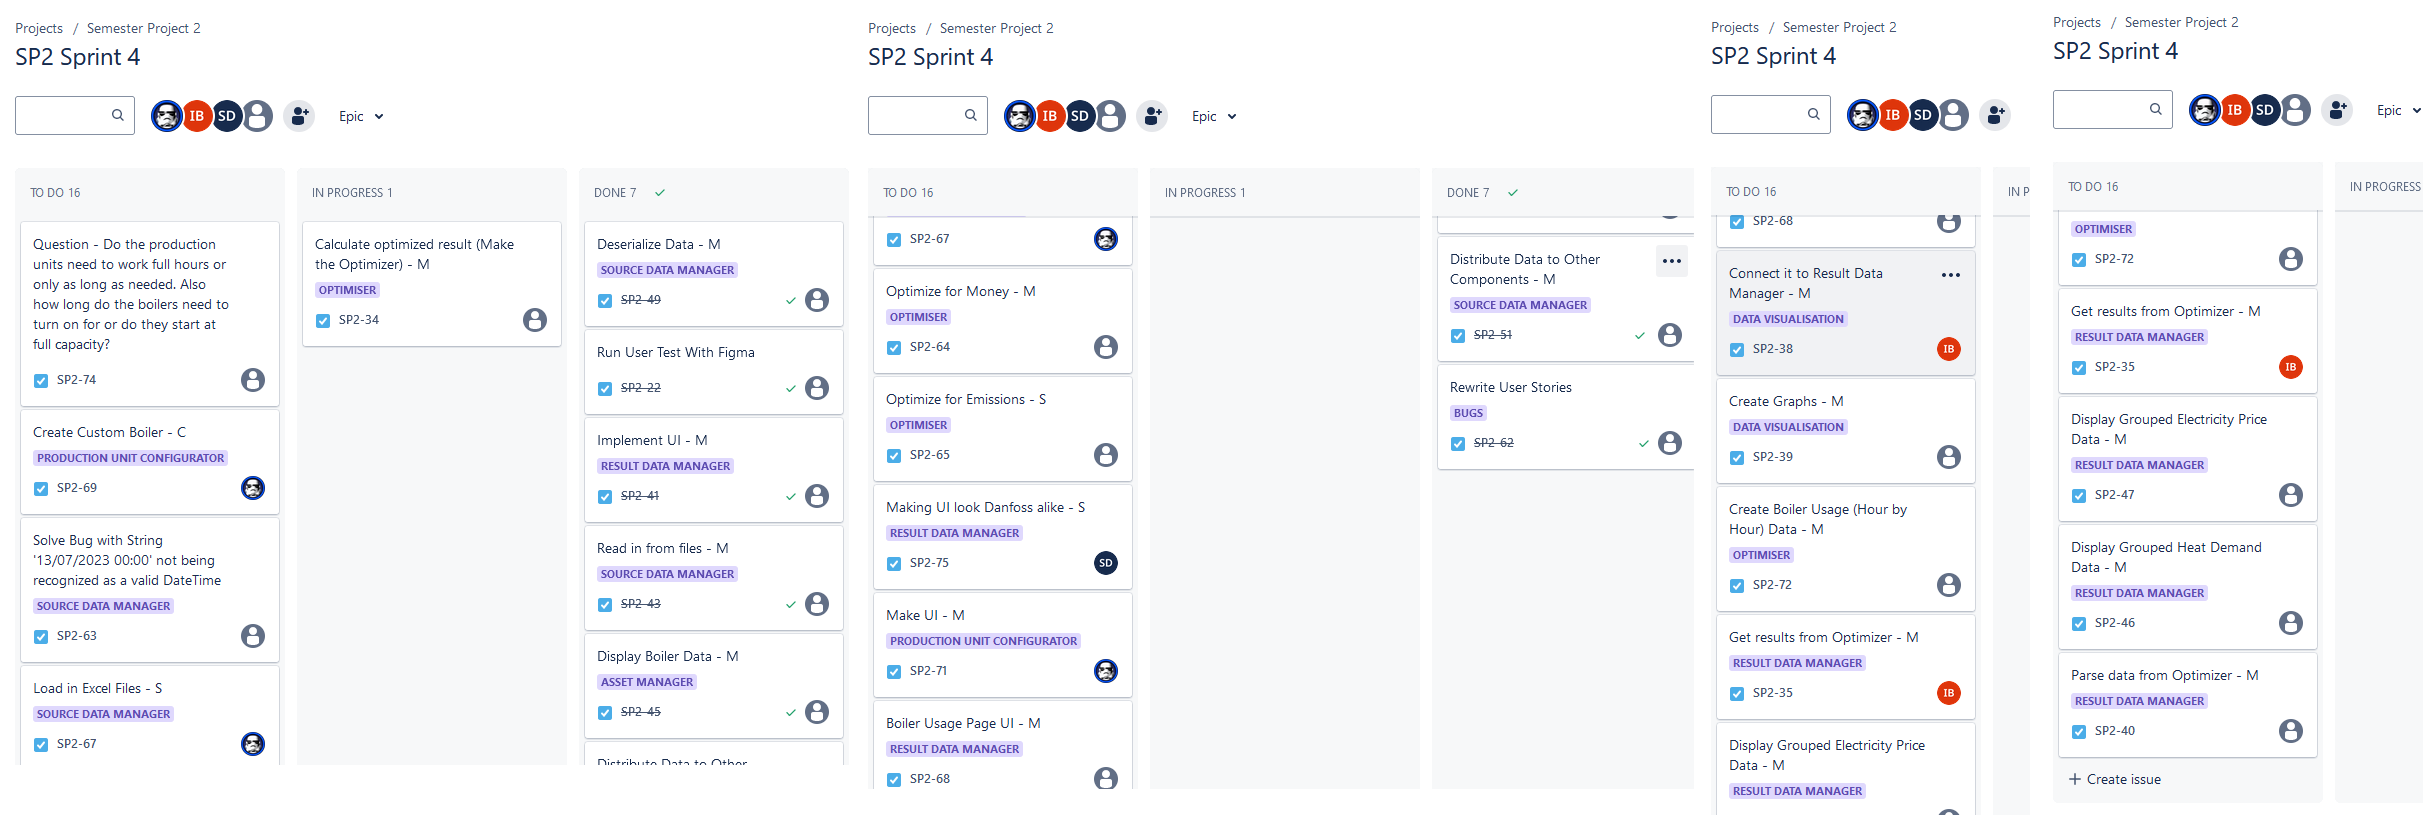
\includegraphics[width=1\textwidth]{Resources/4-Sprint/Daily-Scrum/Backlog.png}
  \caption{Daily Scrum Backlog}
  \label{fig:S4Scrum-image}
\end{figure}
\clearpage

%Review
\subsection*{Sprint Review}
\textbf{Project:} Semester Project Group 11 \\
\textbf{Sprint Duration:} April 23 - May 7, 2024 \\
\textbf{Team Members:} Kacper Grzyb, Sebestyen Deak, Ignat Bozhinov, Leonardo Gianola, Levente Sohar \\
\textbf{Stakeholders:} Sadok Ben Yahia

\subsection*{1. Sprint Goals and Outcomes}
The goal for this sprint was to start fully developing the program. For this, we added every issue that's a must (according to the MoSCoW breakdown we made) for the minimal viable product. We overshot our capabilities on purpose, so we see what to do, and we will continue working on this in the next sprint as well.
\begin{itemize}
    \item \textbf{Goal 1:} Create Comparable Data\\
    \textbf{Status:} Completed. Created two additional classes based on the Optimizer class, that create scenarios which are not the optimal case, to have something to compare our solution to.
    \item \textbf{Goal 2:} Boiler Usage Data\\
    \textbf{Status:} In Progress. The data of which boiler is running when is created, it needs to be grouped and displayed to the user.
    \item \textbf{Goal 3:} Neural Network Optimizer\\
    \textbf{Status:} In Progress. The program is written for a neural engine to find the optimal solution, it just needs to be trained, and then introduced to the project environment.
    \item \textbf{Goal 4:} Create Graphs\\
    \textbf{Status:} To Do. We plan on displaying the different scenarios for the user next to each other in bar graphs.
    \item \textbf{Goal 5:} Choosing Boilers for the Optimization\\
    \textbf{Status:} To Do. We want the user to be able to choose which boilers they want to use to get the optimized results.
    \item \textbf{Goal 6:} Save to CSV files\\
    \textbf{Status:} To Do.
\end{itemize}

\subsection*{2. Completed Work}
The members of the group are focusing on the upcoming Mathematics Exam, not on the project. The next sprint is planned to be more productive. Still, everyone is moving slowly forward with their to-dos. The only task that has been fully accomplished was requested by our supervisor.
\subsection*{3. Unfinished Work}
Many things, including the Data Visualization, Creating and Choosing boilers.
\subsection*{4. Quality and Technical Issues}
All the bugs from the last sprint have been fixed. There are no known issues at the moment.
\subsection*{5. Team Dynamics and Collaboration}
Work has been mostly divided equally, with everyone doing their part. Communication was clear and to the point. We had weekly meetings for scrum.
\subsection*{6. Processes and Tools}
Jira helps keep track of the backlog and manage the sprint. Razor pages and Bootstrap have been used for UI. We sometimes looked back at our Figma prototype for reference.
\subsection*{7. Stakeholder Feedback}
The feedback of our supervisor has been to provide some reference point for the data that our optimizer gives as the end result. This has been mostly accomplished in this sprint.
\subsection*{8. Obstacles and Impediments}
The pressure of the upcoming math test reflected on the amount of work done.
\subsection*{9. Successes and Wins}
There has not been any outstanding win or success during this sprint.
\subsection*{10. Action Items for Improvement}
Pass the exam with good grades, so all energy can be focused on the project.
\hfill 07/05/2024

\begin{figure}[H]
  \centering
  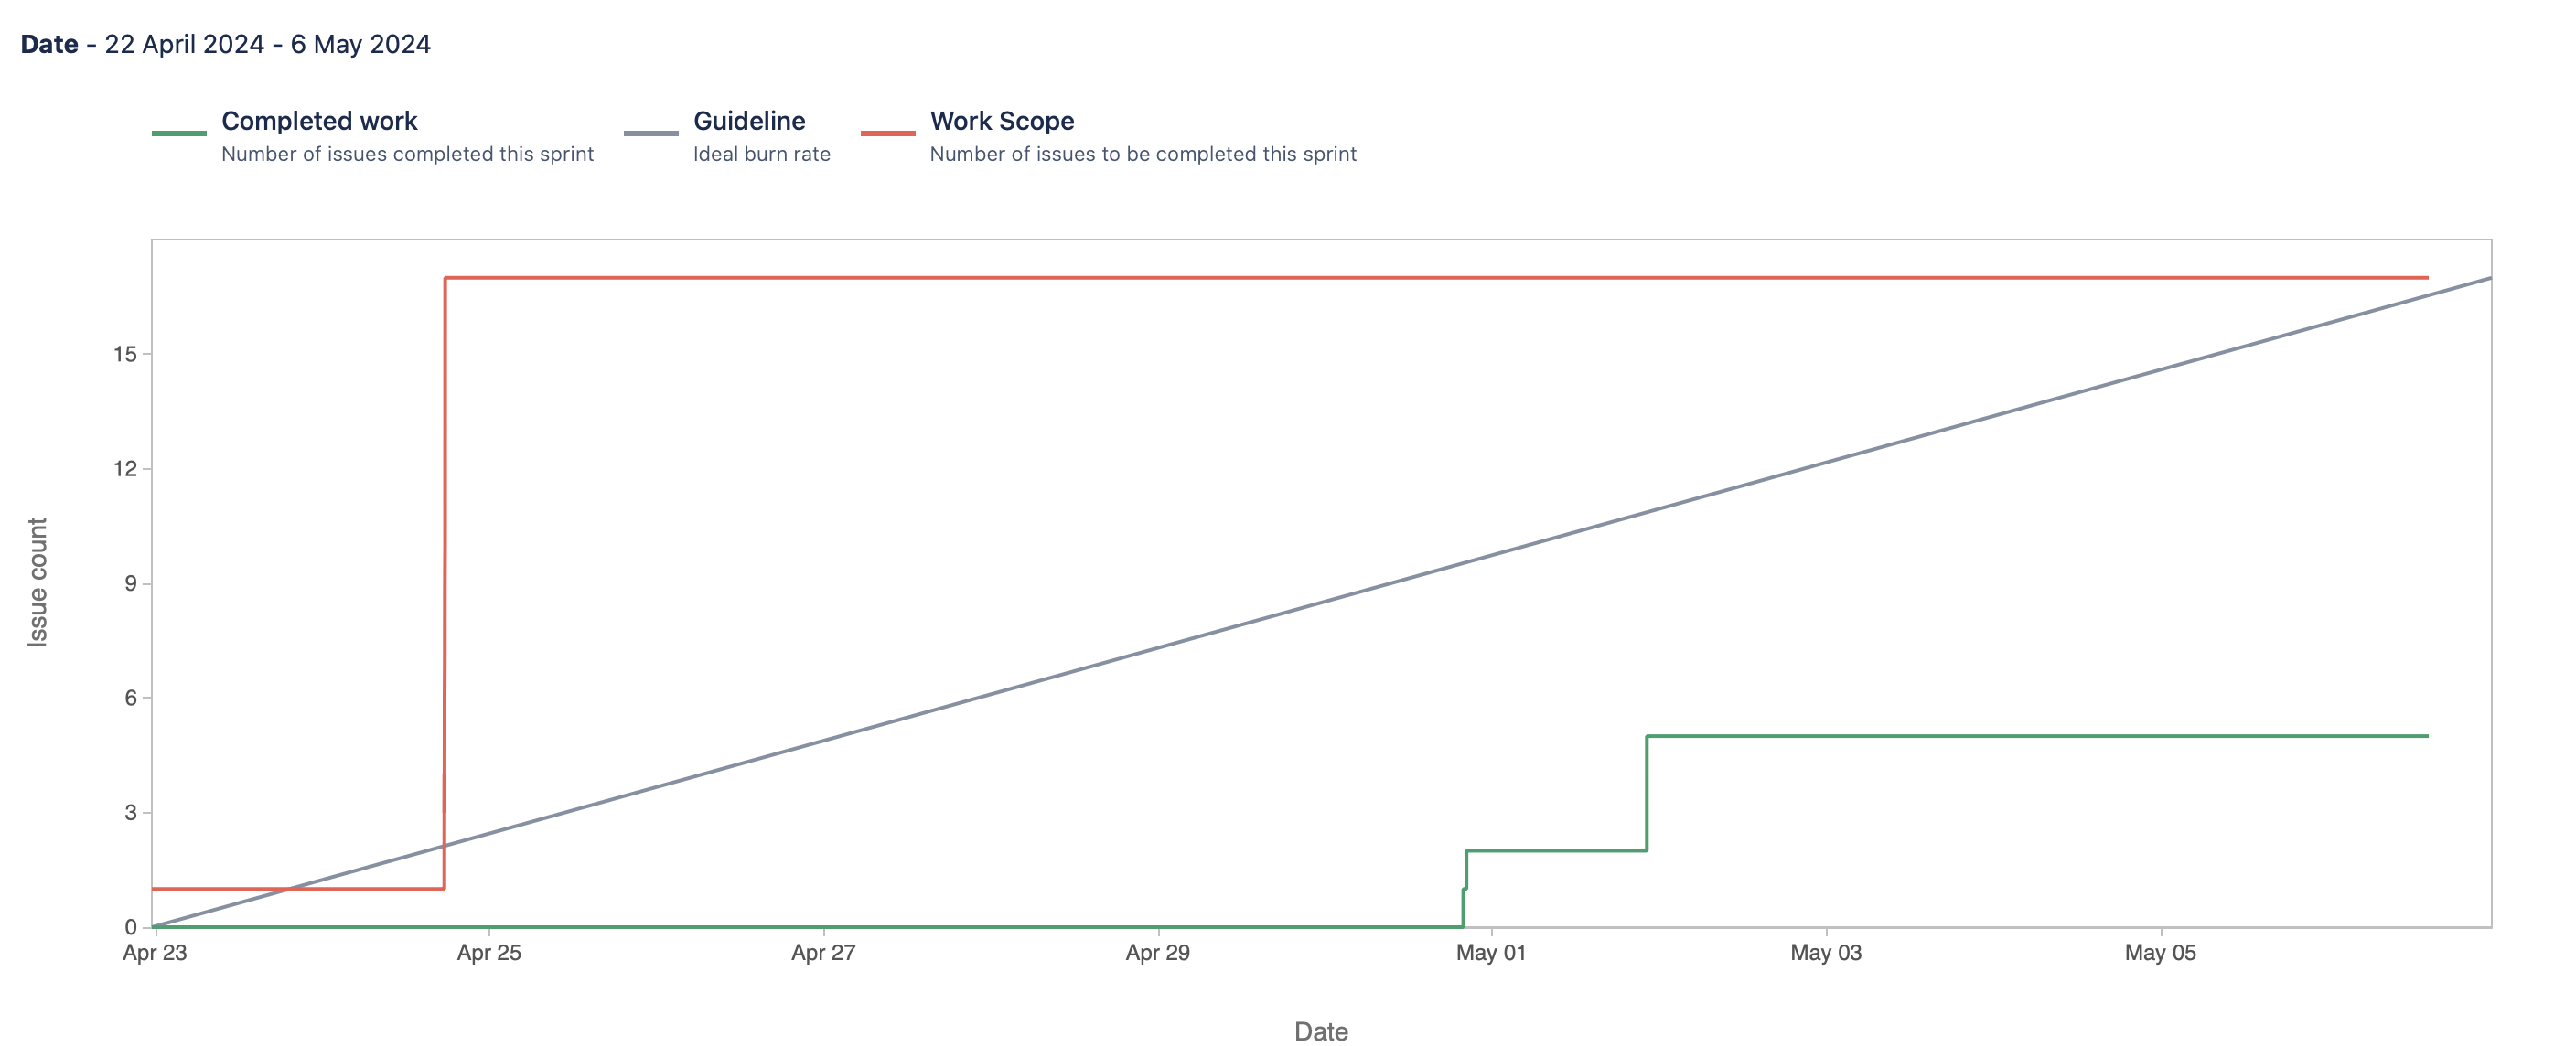
\includegraphics[width=1\textwidth]{Resources/4-Sprint/Review/Burndown.png}
  \caption{Sprint 4 Burnup Report}
  \label{fig:S4Burndown-image}
\end{figure}

\begin{figure}[H]
  \centering
  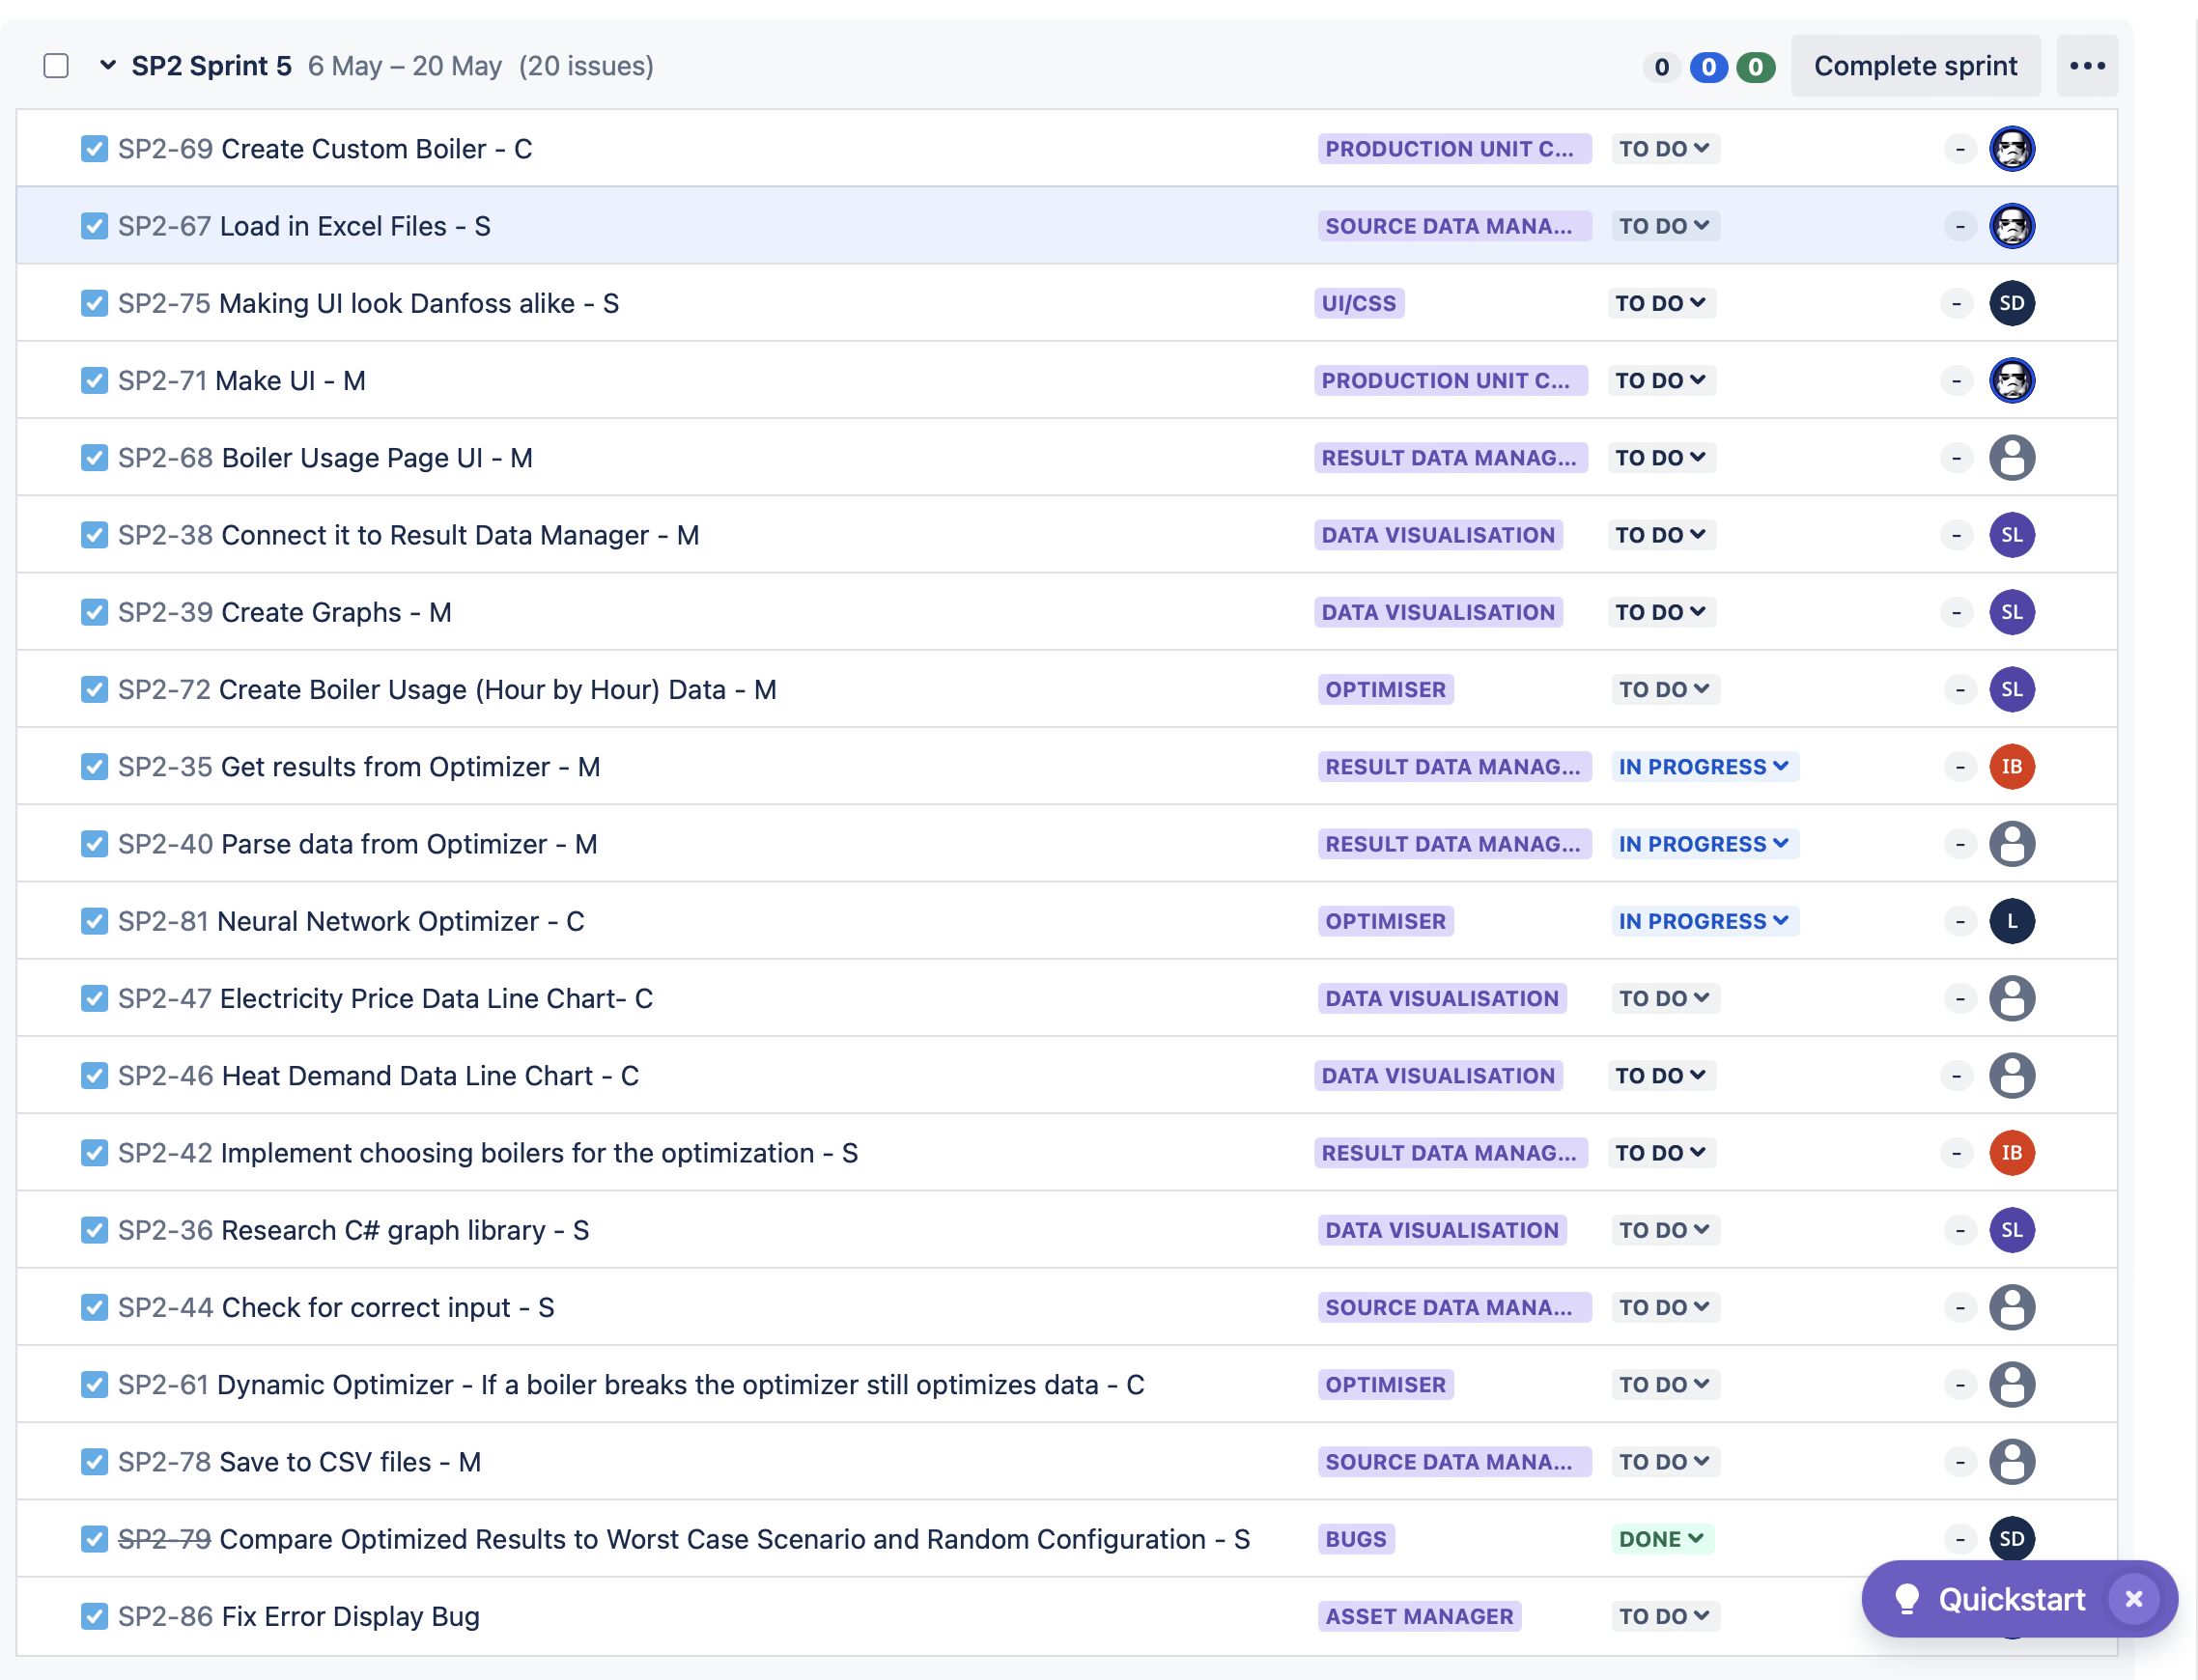
\includegraphics[width=1\textwidth]{Resources/4-Sprint/Review/Issues.png}
  \caption{Sprint 4 Issues}
  \label{fig:S4Issues-image}
\end{figure}
\clearpage







\section {Sprint 5}
%Planning
\subsection*{Planning}
We aim on delivering an almost final version of our product. The Danfoss Demo is going to take place at the end of this Sprint, and we want more than the MVP to be ready by then. We plan on making the Data Visualization with showing the end result and maybe the initial data given in, boiler customization and choosing which one to run for the optimization and a few more smaller things. All members were present on the meeting, and issues have been distributed among us.

\begin{figure}[H]
  \centering
  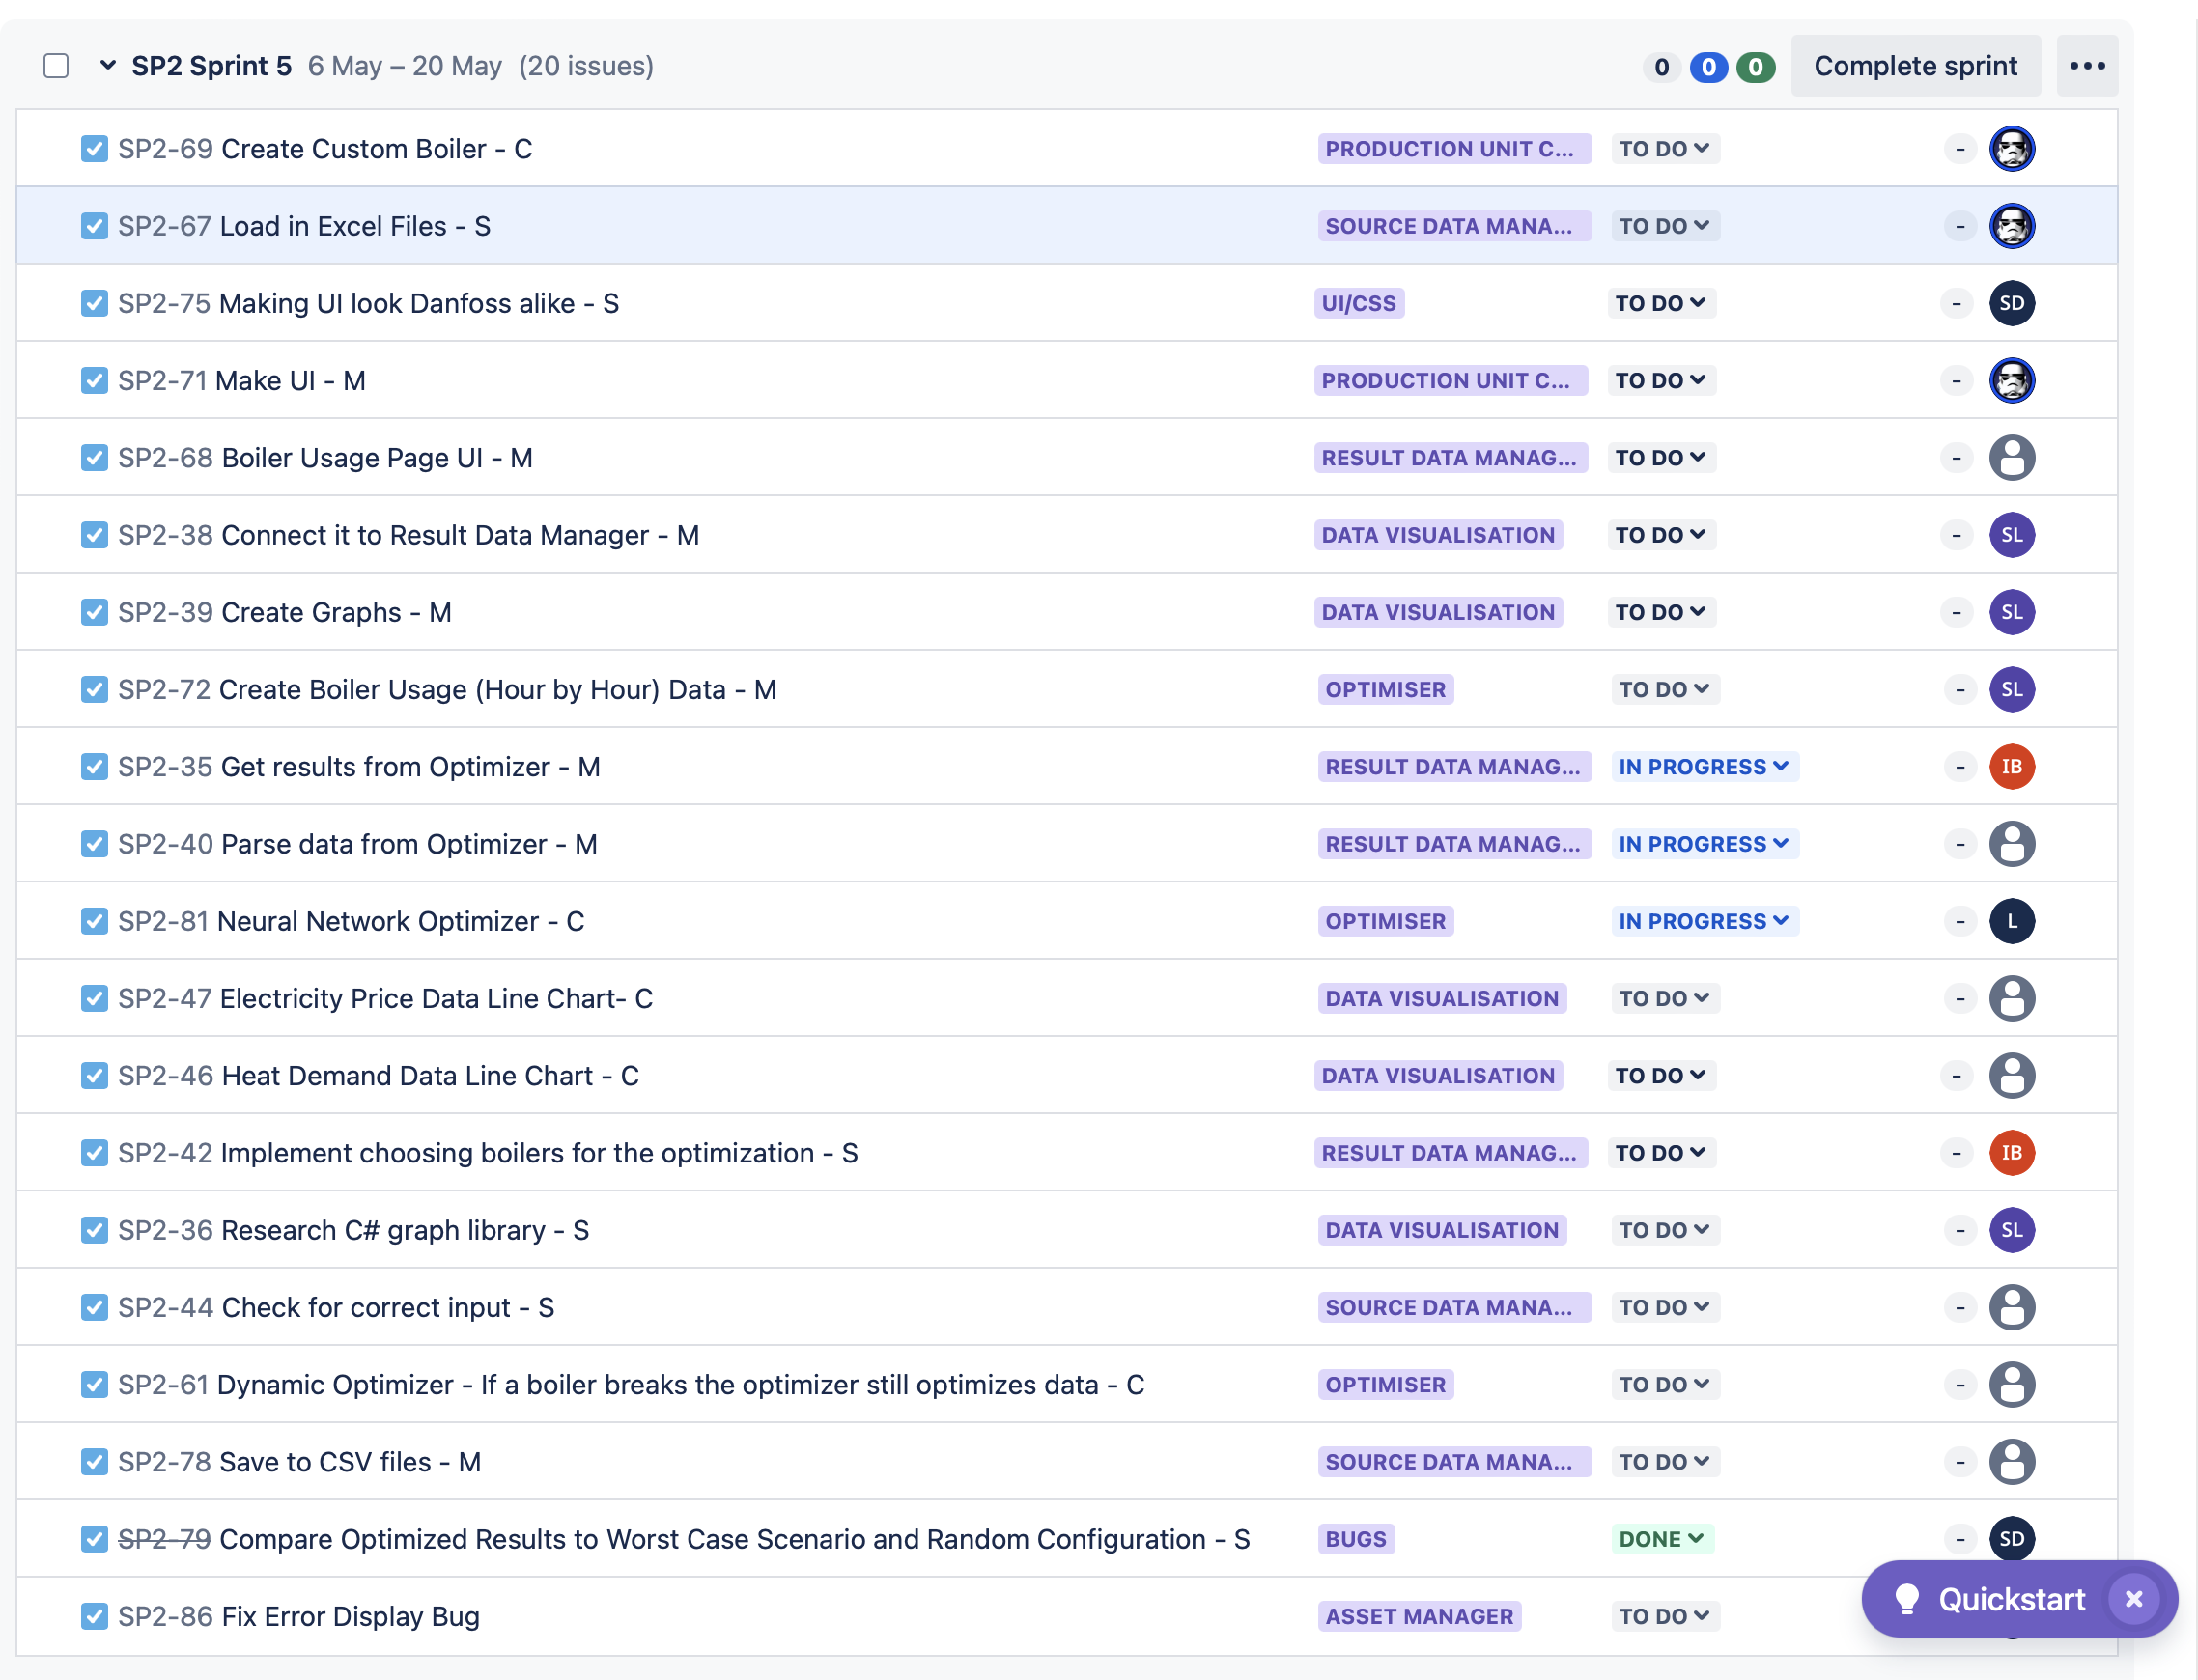
\includegraphics[width=1\textwidth]{Resources/5-Sprint/Planning/Jira.png}
  \caption{Planning Backlog}
  \label{fig:S5Planning-image}
\end{figure}
\clearpage

%Scrum
\subsection*{Daily Scrum 19/05/2024}
\subsection*{Team Update}
\begin{itemize}
    \item The team finished 7 issues and made major progress towards the biggest issue out of the 24 issues in the current sprint.
    \item Leonardo is continuing to work on the Neural Network solution for the optimizer. Levente is making the graphs to show and compare the data from the program. Ignat is finalizing the looks of the pages. Kacper and Sebi are working on being able to read in and to save to different files.
    \item The goal for the sprint is to get as close to the final product as possible for the presentation at the end of this sprint.
\end{itemize}

\subsection*{Roadblocks}
\begin{itemize}
    \item The team was slowed down by the math exam last week.
    \item Every roadblock was talked about and resolved in this meeting.
\end{itemize}

\subsection*{Plans for the Next Sprint}
\begin{itemize}
    \item Because we plan on finishing all the must features next sprint, we plan on polishing any mistakes, and maybe adding a few of the Could features.
    \item Build on the feedback given at the presentation.
    \item Make sure all requested features are accounted for in the sprint backlog.
\end{itemize}

\subsection*{Metrics and Progress}
The team has attached screenshots of Jira for progress metrics.

\begin{figure}[H]
  \centering
  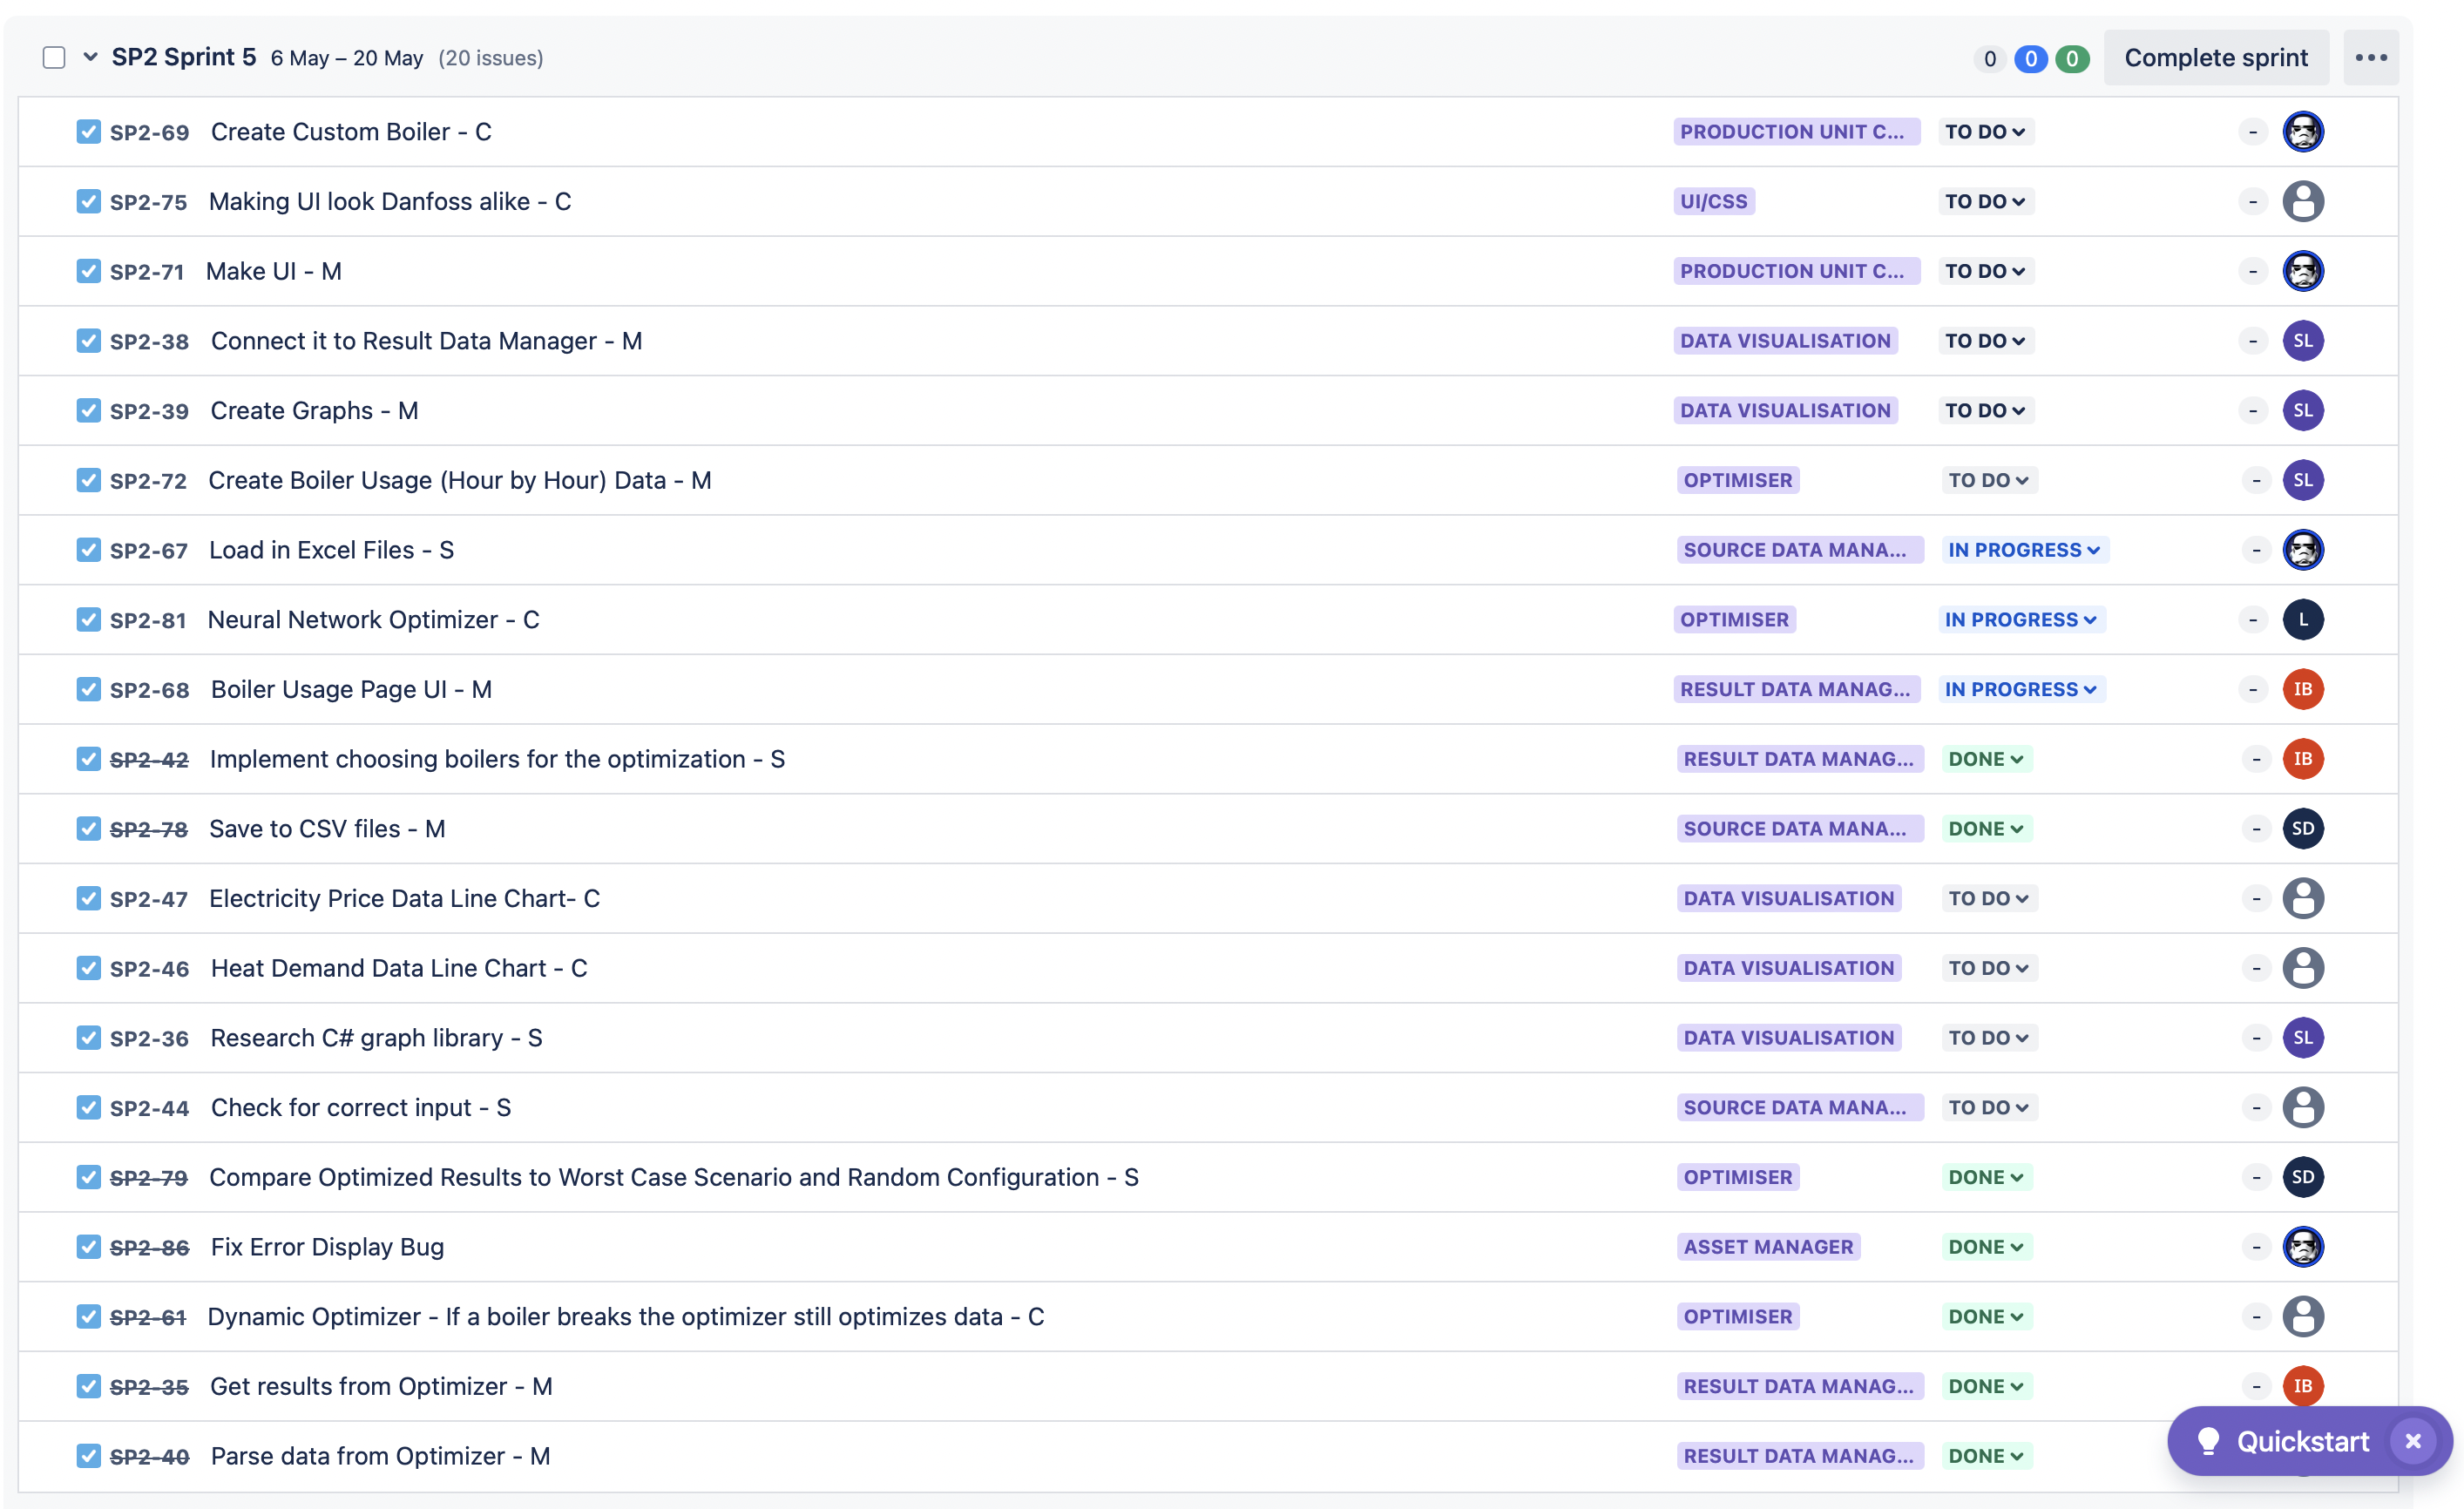
\includegraphics[width=1\textwidth]{Resources/5-Sprint/Daily-Scrum/Jira.png}
  \caption{Daily Scrum Backlog}
  \label{fig:S5Scrum-image}
\end{figure}
\clearpage

%Review
\subsection*{Sprint Review}
\textbf{Project:} Semester Project Group 11 \\
\textbf{Sprint Duration:} May 7 - May 21, 2024 \\
\textbf{Team Members:} Kacper Grzyb, Sebestyen Deak, Ignat Bozhinov, Leonardo Gianola, Levente Sohar \\
\textbf{Stakeholders:} Sadok Ben Yahia

\subsection*{1. Sprint Goals and Outcomes}
The goal for this sprint was to finish developing the program's must-have features and polish them to be acceptable for the presentation. We carried on with the remaining tasks from Sprint 4 and continued the development of the full program.
\begin{itemize}
    \item \textbf{Goal 1:} Create Boiler Usage\\
    \textbf{Status:} Completed. Created an additional page inside the program, where the distribution amongst boilers can be viewed, in addition to the saving options.
    \item \textbf{Goal 2:} Create Custom Boiler\\
    \textbf{Status:} Completed. The user of the program can now create a fully customizable boiler.
    \item \textbf{Goal 3:} Neural Network Optimizer\\
    \textbf{Status:} Completed. The program is written for a neural engine to find the optimal solution.
    \item \textbf{Goal 4:} Create Graphs\\
    \textbf{Status:} Completed. All vital and comparable data is displayed for the user to put the optimized scenario in context.
    \item \textbf{Goal 5:} Choosing Boilers for the Optimization\\
    \textbf{Status:} Completed. We made it possible for the user to choose which boilers they want to use to get the optimized results.
    \item \textbf{Goal 6:} Save to External Files\\
    \textbf{Status:} Completed. The user is now able to save the boiler usage and the optimized data to external CSV and Microsoft Excel files.
    \item \textbf{Goal 7:} Heat Demand and Electricity Price Line Chart\\
    \textbf{Status:} To-Do. We want to display additional information about the provided data to give a deeper understanding to the user.
\end{itemize}

\subsection*{2. Completed Work}
Many things have been completed during this sprint, all big steps towards the end goal. The biggest things are the new UI of the application, saving to files, and making custom boilers.
\subsection*{3. Unfinished Work}
Not that many things remain, essentially all the must-have features from the MoSCoW breakdown have been created.
\subsection*{4. Quality and Technical Issues}
The graphs don't display correctly from time to time, but the bug can be resolved by reloading the page.
\subsection*{5. Team Dynamics and Collaboration}
Work has been mostly divided equally, with everyone doing their part. Communication was clear and to the point. We had weekly meetings for scrum.
\subsection*{6. Processes and Tools}
Jira helps keep track of the backlog and manage the sprint. Razor pages, Bootstrap, and JavaScript have been used for UI.
\subsection*{7. Stakeholder Feedback}
There hasn’t been much feedback after the presentation.
\subsection*{8. Obstacles and Impediments}
None noted.
\subsection*{9. Successes and Wins}
The presentation was a great success, and the program is almost finished.
\subsection*{10. Action Items for Improvement}
None noted.
\hfill 22/05/2024

\begin{figure}[H]
  \centering
  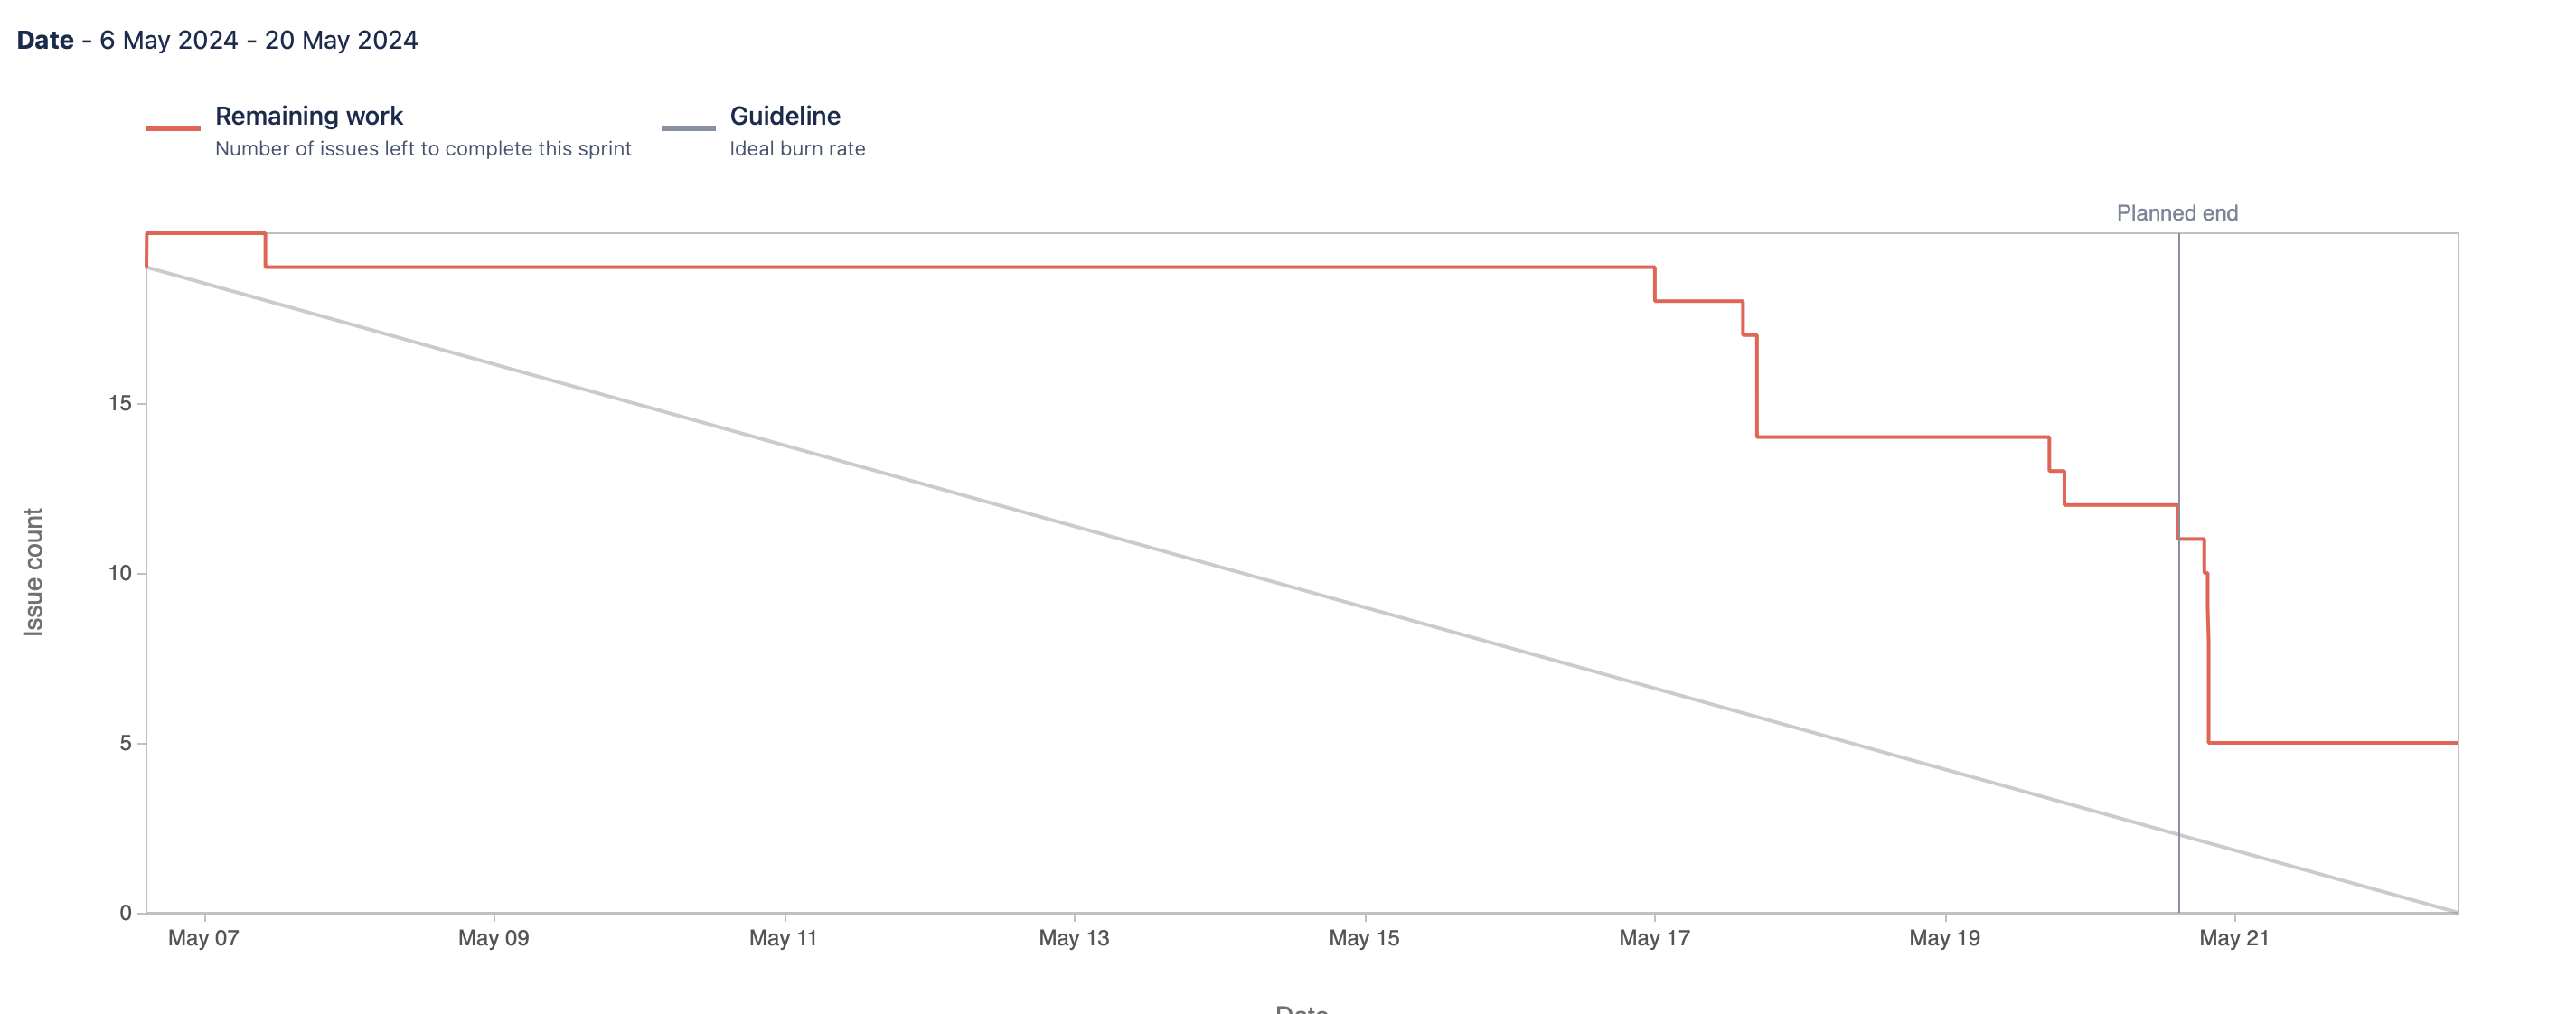
\includegraphics[width=1\textwidth]{Resources/5-Sprint/Review/Burndown.png}
  \caption{Sprint 5 Burndown Chart}
  \label{fig:S5Burndown}
\end{figure}


% Chapter 4
\chapter{Technical Details}

% Chapter 4a
\section{Software Architecture and Design}

\subsection*{Tools}
The team decided to use the ASP.NET Core framework's Razor Pages for building the project for reasons such as:
\begin{itemize}
  \item The most important argument for using ASP.NET Core is it's cross-platform functionality. The developers in the team use 
  both Macintosh and Windows based systems, therefore a framework that could switch seamlessly between them was crucial.
  \item As the name suggests, the framework runs in the .NET ecosystem, which is what the team has been taught in the course so far
  therefore it is what the team is most experienced and most comfortable working in.
  \item With Razor Pages being a web-page based solution, the UI is mostly composed of HTML and CSS, which some team members already
  had experience in and the rest was eager to learn. A light-weight, web-based solution allowed the team to be more flexible,
  and develop the app at a more rapid pace compared to if the team chose a Model-View-Controler (or a Model-View-ViewModel) solution.
  This freedom allowed for more features and made the process of adjusting to changing the project requirements easier.
  \item Additionally, Razor Pages allows the project to be published and deployed straight away, which is a nice bonus.
\end{itemize}
As for other tools, the team used:
\begin{itemize}
  \item Github: Source and Version Control, Collaborative Development of the App
  \item Jira: Task Management and Planning as well as adhearing to Agile which was one of the requirements for the project
  \item Discord: Communication and Resource Sharing
  \item diagrams.net|draw.io: Creating UML Diagrams 
  \item Figma: Prototyping and General UI Design
  \item Visual Studio and Visual Studio Code: Code Editors
\end{itemize}


\subsection*{Application Flow}
\label{sec:appflow}
The user journey begins in the Homepage, which is the project requirements' Asset Manager component. The user inside of this component has two possible routes:
\begin{itemize}
  \item Load Heat Demand Data
  \item Configure Production Units
\end{itemize}
Let's explore unit configuration first. When the user clicks on that option, they get redirected to the unit configuration page, where they
can change the properties of the pre-loaded production units provided by the project requirements (Gas Boiler, Oil Boiler, Gas Motor and Electric Boiler), while
also being able to create and configure thier own custom production units. From this page the only option is to go back to the Homepage.
Next, loading the heat demand data can be done in one of three ways: choosing the preloaded data provided by Danfoss Deliveries 
(Winter Period Heat Demand 08.02.2023-14.02.2023 and Summer Period Heat Demand 08.07.2023-14.07.2023), loading the data from a custom CSV file or loading the data from a custom Excel Workbook file.
Once heat demand data has been loaded, more options open up for the user in the navbar:
\begin{itemize}
  \item Database Preview
  \item Result Data Manager
\end{itemize}
The Database Preview component was not initially intended to stay in the final product. At first it was used solely for debugging purposes, when 
the team was implementing the data loading options. But due to supervisor and project presentation feedback, we decided to keep this component
to also allow the user to double-check if their data was correctly loaded and recognized by our application. From this page the user has the option to either
go back to the Homepage or go to the Result Data Manager.

The Result Data Manager is where the magic happens. It hosts the main functionality of the program which is the Optimizer Component, Data Visualization and saving optimized data.
By default, the Optimizer runs automatically whenever the user get redirected to this page with the settings: Use all production units,
optimize for costs, use the standard optimizer. We made this choice so that the user is immediately greeted by the results, and not just a blank page.
Once on the page, the user can tune the optimizer to produce data that suits their individual needs. Here are the checkbox options given:
\begin{itemize}
  \item Choose which production units to include in the optimization process
  \item Choose which parameters to optimize for (Costs, CO2 Emissions)
  \item Choose which optimizer to use (Standard or Neural Network)
\end{itemize}
Then the user can rerun the optimization process with the selection options to obtain their results. The results themselves are displayed in the same page,
both in text and graph format, which covers the data visualization requirement. Having the optimization outcomes opens up some more paths to take:
\begin{itemize}
  \item Unit Activations Page
  \item Save Optimized Data to CSV
  \item Save Optimized Data to an Excel Workbook
\end{itemize}
The Unit Activations Page is the last component the user gets access to in their journey. It shows the activation percentages for each production unit at each timeframe.
They can be treated as instructions for the user on how to manage the boilers to achieve the optimal Produced Heat, Electricity Consumption, Production Costs, 
Fuel Consumption and CO2 Emissions proposed by the current optimizer configuration.
The last options allow the user to save all of the optimizer output data mentioned previously into a single CSV or Excel Workbook file, which gets
downloaded to the users Downloads folder.


The project in itself does not operate on many states, therefore it does not need nor have a complex state machine diagram.
Most of the application's functionality happens automatically and/or instantly, therefore creating custom states and switching between them
would have created unnecessary complexity and slowed down the program. With that in mind, during the creation of the state machine diagram,
we decided to focus on how Razor Pages functions in general, where the main states are waiting for post requests which is, in other words, user input.
Despite that, we still thought that a state machine diagram was one of the best ways to represent the application flow and user journey
therefore it can be seen below.

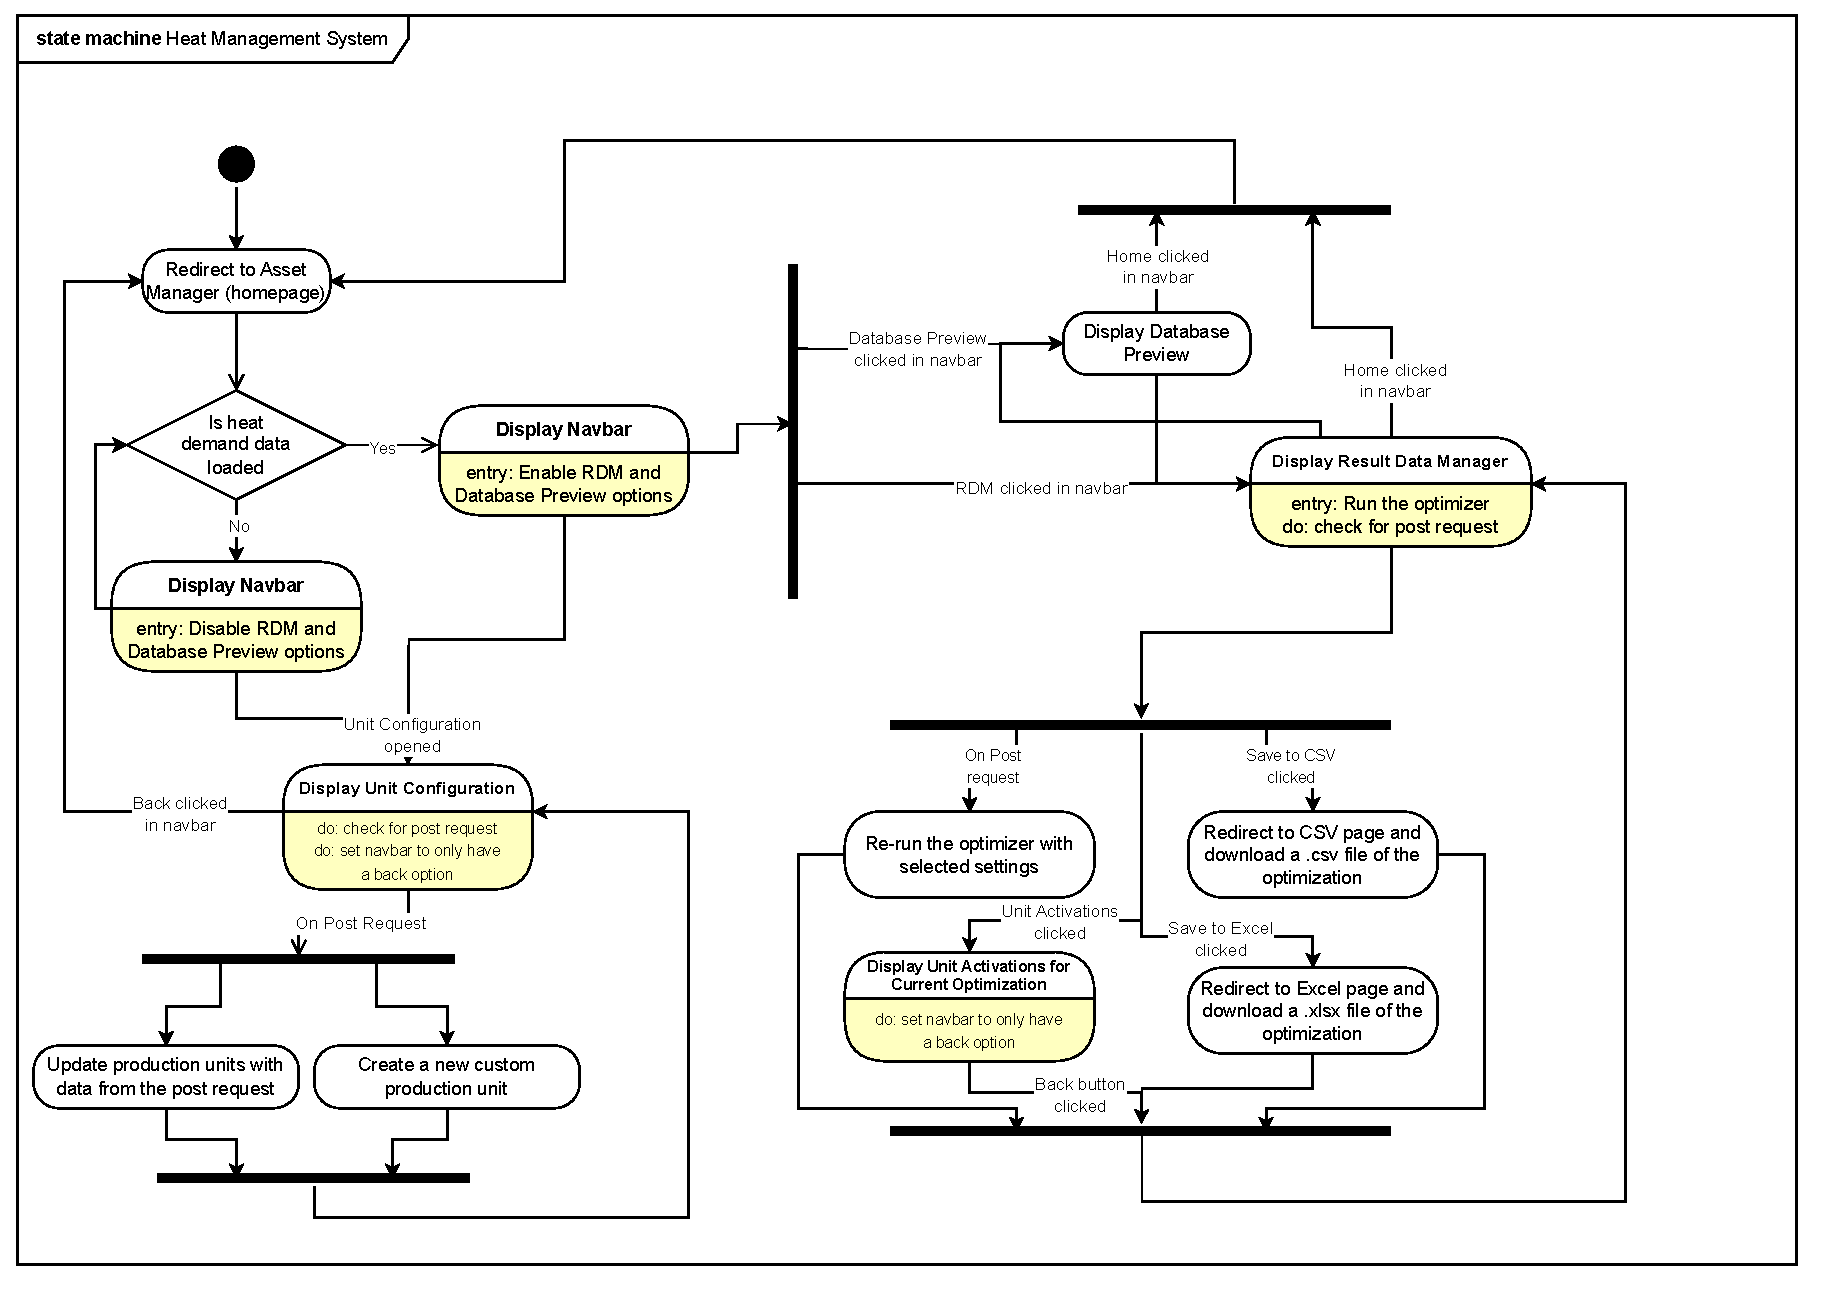
\includepdf[pages=-]{Resources/SP2-state-machine.pdf}


\subsection*{Database Design}
\label{sec:database}
Before diving into the program architecture the in-memory database solution offered by Razor Pages must first be mentioned.
In order to achieve data persistance while switching in between pages in a Razor Pages project, a database must be used. 
Since we did not want to go too far out of the scope of the project, we decided not to use a dedicated database solution
like a MySQL or MSSQL Server for this project, expecially because the team has not had any database modeling courses
yet. Instead we chose a middle-ground, which is the before mentioned in-memory database. This soultion offers similar functionality
to a real database, with the comfort of running in the program's memory, which eliminates potential connection, authentication
privilege and/or security risks and issues connected with using databases. To represent the applications data storage sytstem
the group devised an improvised custom uml diagram inspired by other standardized database diagrams. It can be seen below, together with
explanation for each of the tables.

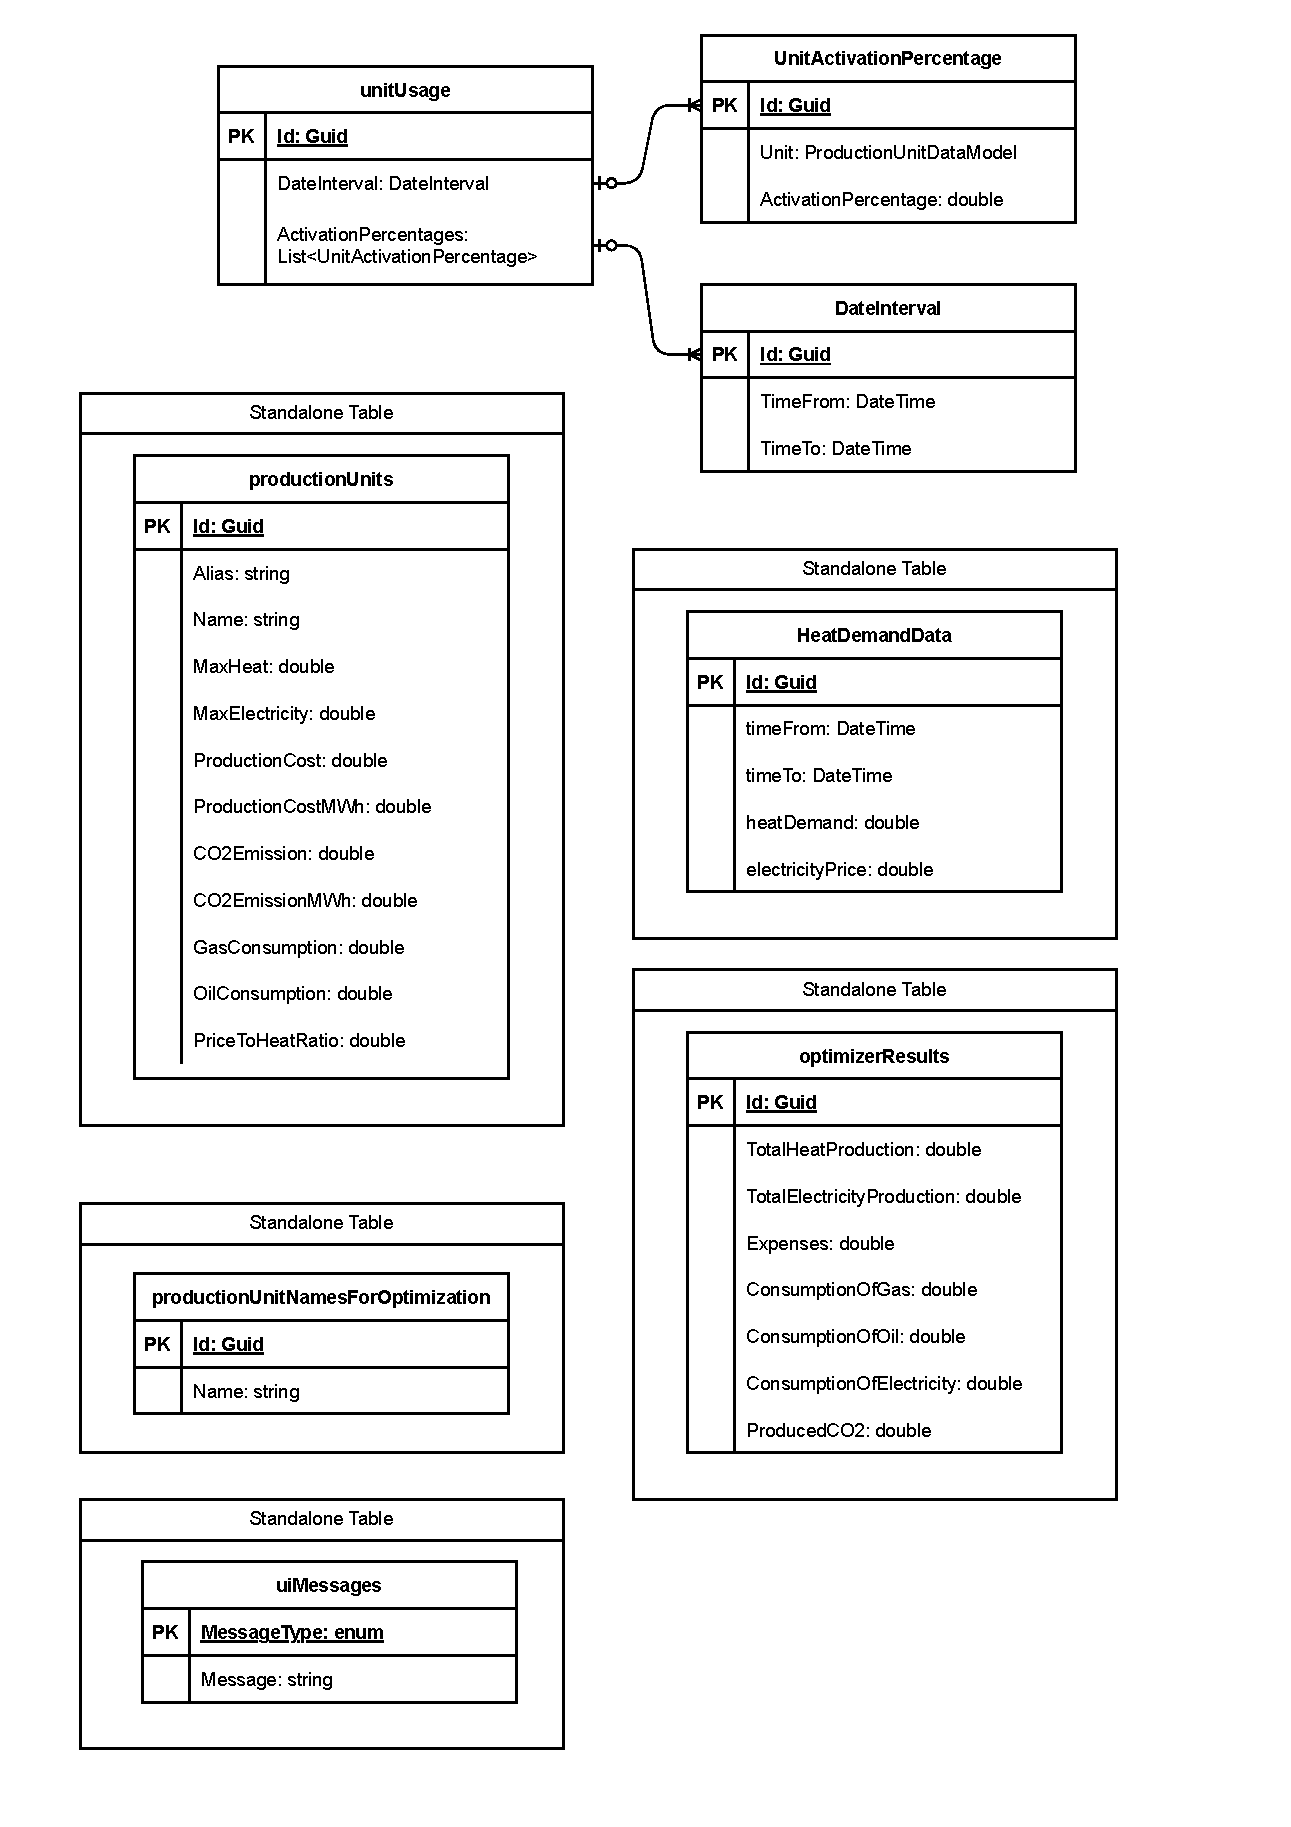
\includepdf[pages=-]{Resources/SP2-database-diagram.pdf}

The database does not fully comply to database system standards. 
We do see the limitations and flaws of this design choice, such as the lack of connections between tables and the 
lack of foreign keys inside of each table. Instead some fields in the tables use custom class data types for ease of use. Despite the flaws
of using DbSets, we found that their functionality was sufficient for the scope of the project. It is also worth to mention, that due
to our lack of experience with Razor Pages, we were unsure of how DbSets and in-memory data structures function. Because of that in the
middle of development the database had to be refactored from a more json-like data storage structure to one that complies
with standards enforced by DbSets, such as using Primary Keys. It is because of this process that we ended up having a mixture of both structures.
The most crucial tables found within the programs database are the \textit{productionUnits} and \textit{HeatDemandData}. As the names suggests
they contain data that is needed for the application's main functionality - calculating optimized production unit usage results for 
the inputted heat demand for each timeframe. Some of the properties inside of \textit{productionUnits} are additions from the team, such as
\textit{ProductionCostMWh} and \textit{CO2EmissionMWh}, which made it easier to remember how to calculate final optimization results, and
\textit{PriceToHeatRatio}, which also was a helper variable in optimization calculations.
When it comes to storing the results from the optimizer for later display or download, the \textit{unitUsage} and \textit{optimizerResults} tables were used.
We think their names explain their functionality sufficiently.
Lastly, the \textit{uiMessages}, as the name suggests stores messages for the user that may appear in the user interface under certain conditions, such as 
confirmation of a successful data upload or an error during the optimization process.
These messages have to be stored in a database, because of how user input works in Razor Pages. The only way the team found to obtain user input is through
post requests, which only make impact on the interface after a page redirect, which would reset the pages memory and lose the message intended for display.
That is why for these messages to persist it is important to have a place to save them before the redirect.


\subsection*{Code Architecture}
\label{sec:code}
With the database covered, we can shift our focus towards the rest of the codebase. Any issues, bugs or problems encountered
by the group during the development/implementation phase of the project will be \underline{underlined} in this subsection of the report.
We shall start in the same place as the program's structure: \textit{Program.cs}. This file mostly contains
automatically generated Razor Pages setup code for every built-in feature to work correctly, but it is also where one of the first problems started.
\underline{Culture Info} was a common problem across all groups working on this project in this semester, and it definitely caused some issues for us as well,
like incorrect DateTime variable parsing, incorrect decimal separator detection, errors with reading data from files and incorrect data display.
Fortunately manually setting the user's DefaultThreadCurrentCulture and DefaultThreadCurrentUICulture to the Danish CultureInfo
was an easy fix that solved most of these problems. From this code file, the Razor Pages applications gets built and the user gets redirected
to the \textit{Index.cshtml} page with the Navbar and DataUpload ViewComponents overlayed on top of it, which we will come back to shortly.
The group chose to create both component and class diagrams to explain how the code is designed. The component diagram helps us break down
the program into the components from the project's requirements, and clarify in which location each component is implemented.
This diagram also plays a part in explaining the interactions between each component, and the class diagram is able to complete this explanation,
as well as go more in depth for each component, breaking them down into individual classes. The component diagram can be seen below.

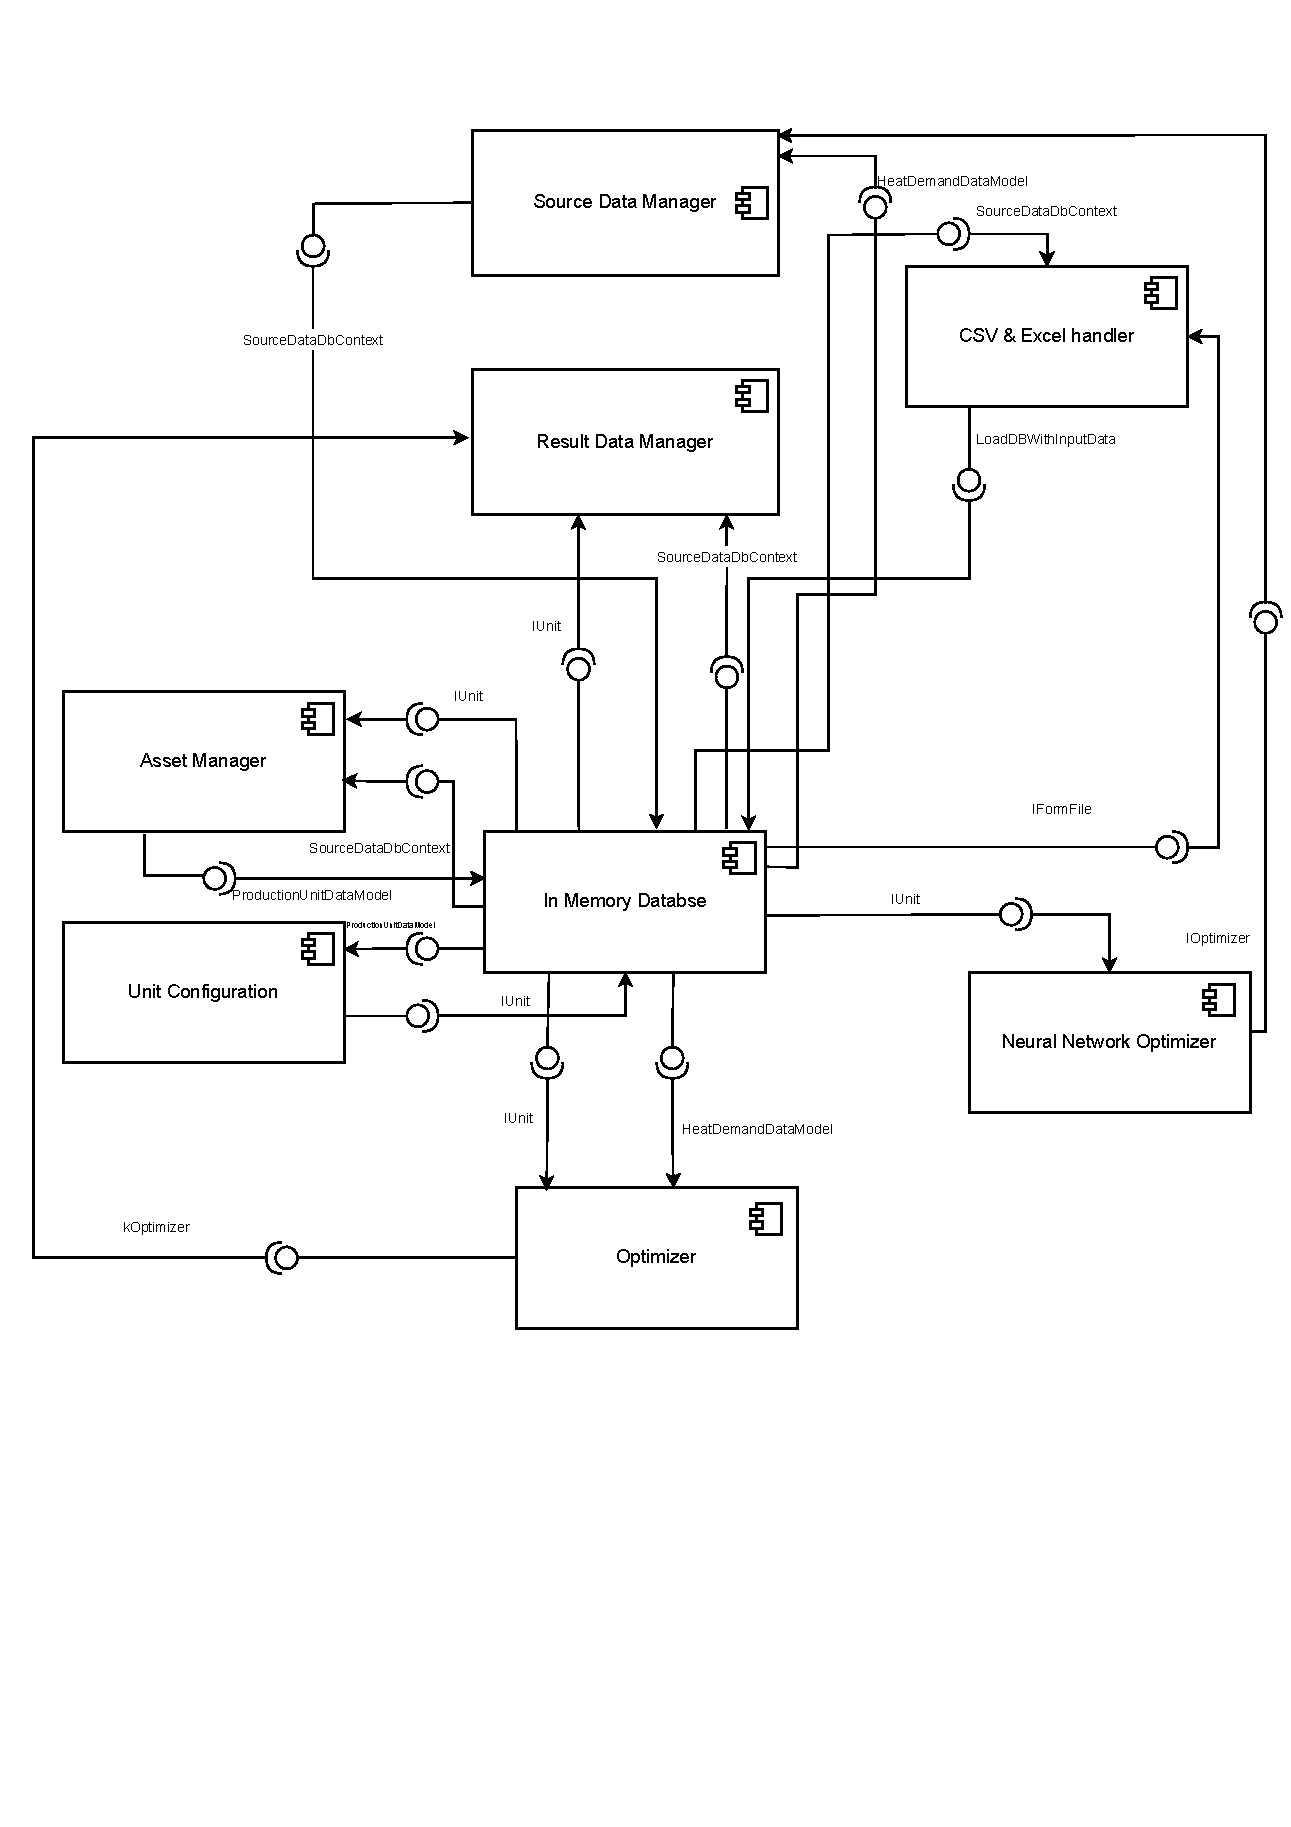
\includepdf[pages=-]{Resources/SP2-component-diagram.pdf}

Following the component hierarchy we will cover the \textbf{Source Data Manager} next. The class diagrams facilitating this explanation
can be seen below this paragraph. Our implementation of this component makes it handle the most important interaction between the program
and the database, which is loading user input or pre-loaded data and deleting that data. The component itself is an 
implementation of the \textit{IDatabaseManager} interface, which was used to reinforce the SOLID principles within our codebase,
decouple dependencies, make the code less brittle and more expandable. The main property of \textbf{Source Data Manager} is \textit{\_context},
which will appear in most other components, and is essentially a reference to the in-memory database. \textit{SourceDataDbContext}, which
implements the \textit{DbContext} Interface is the class that contains the in-memory database. It uses class data models such as 
\textit{HeatDemandDataModel}, \textit{ProductionUnitDataModel}, \textit{OptimizerUnitNamesDataModel}, \textit{UnitUsageDataModel},
\textit{UiMessagesDataModel} and \textit{OptimizerResultsDataModel} for data storage. The other properties it contains have custom get and set methods
defined which interact with their respective DbSets, and serve as quick references to specific items from the database that are widely used throughout the program.
This is a result of \underline{major database} \underline{refactor}, before which these properties were preset in the \textbf{Source Data Manager} component.
In order to avoid merge conflicts and errors these properties were kept but puerly as references to the database, which is where
C\#'s feature of custom property getters and setters came in really handy.
Moving onto the \textbf{Asset Manager} component, which uses the \textit{IndexModel.cshtml.cs} class as it's code-behind. As mentioned
previously, this is the Homepage of the program, it contains a reference to the database, OnGet and OnPost methods for handling user
input.
In this component, we also made use of Razor Pages' View Component feature, which essentially allowed us to display a page within
another page, which helped break up the code into more manageable chunks and work on different parts of the page without interfering with each other.
The only two View Components in the program are:
\begin{itemize}
  \item DataUploadView - a page that either calls \textbf{Source Data Manager} to load in pre-provided heat demand data,
  or accepts a file uploaded by the user, while checking if its format and extension is correct.
  \item PageNavigationView - as the name suggests, it is an overlay that allows the user to navigate through the program, namely
  to three components: \textbf{Asset Manager}, \textbf{Result Data Manager} and \textbf{Database Preview}. The navigation bar is displayed
  in each mentioned component.
\end{itemize}
The \textbf{Asset Manager} also gives access to the \textbf{Production Unit Configuration} component. This is where the user
can configure properties of pre-existing or custom added production units. All of the user input is again handled in the OnGet and OnPost methods
with the aid of the \textit{PUCButtonRequest} class, which allows the OnPost request to recognize which button in the UI was pressed
and to react accordingly. Unit creation, updating and deletion processes use unit IDs from the \textit{ProductionUnitDataModel} class
to make sure changes occur to the right unit, thanks to Guid ensuring each Production Unit record in the database has a unique ID.
Obtaining the new parameters for chaning a picked production unit is handled thorugh binding the \textit{formProductionUnit} property, which is
a technique used also in other pages when handling user input. This is also where an issue came up connected with
\underline{Culture Info}, that was not solved in \textit{Program.cs}, which were the decimal separators for number inputs.
This is why a custom \textit{DoubleModelBinder} was written, to convert HTML form input's values to variables of type \textit{double}
no matter if they used a dot or a comma as their decimal separator. A safety check was also implemented, so that a production
unit's Alias property has to be unique, to eliminate potential errors with the optimization process, which will be covered soon.

\includepdf[pages={4, 1}]{Resources/SP2-class-diagrams.pdf}

Back in \textbf{Asset Manager}, the navbar allows the user to navigate to the \textbf{Result Data Manager} and \textbf{Database Preview}
components. The latter does not contain any distinguishing code, and was covered entirely in the subsection \hyperref[sec:appflow]{Application Flow}.
The \textbf{Result Data Manager}, on the other hand, is the most substancial component of the whole application. The code-behind for its page
is in \textit{ResultDataManagerModel.cshtml.cs}. It contains the usual reference to the database, but a thing that stands out
are the two IUnit Lists and the IUnit Interface itself. Firstly, the program contains both a IUnit Interface and a ProductionUnitDataModel parent class
for production units, which are used interchangeably, because of a \underline{DbSet issue}. At one point in the development
when trying to access one of the feature of DbSets, it turned out that a DbSet cannot be of an interface type. At that point, the IUnit
interface was used extensively within the codebase and there was not enough time to make the changes necessary, so a band-aid fix was applied, with which
the ProductionUnitDataModel class was created. The \textbf{Result Data Manager} also hosts the \textbf{Optimizer}
component, which consists of the KOptimizer, SOptimizer, GeneticAlgorithm (The Neural Network Optimizer) (and WorstScenarioOptimizer with RandomOptimizer, which
are used solely as comparison data for some of the graphs). Multiple Optimizer implementations are a result of one of the
\hyperref[sec:sprints]{Sprints} the team carried out, where everyone worked on an implementation and at the end the best one was chosen.
The main optimizer that the application uses is the KOptimizer, which is also referred to as the Standard Optimizer. It is a simple
Greedy Algorithm implementation that judges which production units are the most cost effective for each timeframe, and uses 
them to produce as much heat as possible until the demand is met. An outlier to the goal of our optimizer sprint was the Neural Network Optimizer,
which was too good of an idea to pass up on, while begin to risky to be the only optimization algorithm, so we decided to use both.
The explanation on how it is implemented can be found in \hyperref[sec:nnexplanation]{Chapter 5c}.
The Optimization Process has 3 main configuration options to consider before re-running it, which were also mentioned in \hyperref[sec:appflow]{Application Flow}.
This configuration is handled in the OnPost method of ResultDataManagerModel. It is important to mention, that due to \underline{allowing}
\underline{the user to choose their own production unit scenario}, each \textbf{Optimizer} implementation had to have a built-in check to
make sure that the production units provided can even meet the heat demand. If that is not the case, the uiMessages
DbSet is used in the database to display an error message to the user.
Additionally, this option meant that we needed to store all of the production units and the production units selected for 
the optimization process by the user at the same time. This is where a second \underline{problem with DbSets} came up.
Razor Pages does not seem to allow for two DbSets of the same type to exist within one database, instead
merging them into one singular DbSet if that was the case, resulting in duplicate key value errors. A workaround had to be implemented.
This is why the OptimizerUnitNamesDataModel exists, which stores just the production unit aliases, which are then matched
with the prodcution units in the productionUnits DbSet and passed into the \textbf{Optimizer}. This is also why the \textbf{Unit Configuration}
component makes sure that each alias is unique.
Once the optimization process is finished, the \textbf{Result Data Manager} saves the outputs to the database using
the UnitUsageDataModel and OptimizerResultsDataModel classes. This is what later allows the ExcelWriter and CSVWriter classes
to access this data, convert it to their own respective formats, and redirect the user to a file download page.
Lastly, \textbf{Result Data Manager} also hosts the \textbf{Unit Activations} component, which in similar fashion
as the \textbf{Database Preview}, was covered in \hyperref[sec:appflow]{Application Flow}.

\includepdf[pages={3, 2}]{Resources/SP2-class-diagrams.pdf}

% Chapter 4b
\section{Simple Design}
In software engineering, simple design is a fundamental element to creating a software. The aim of this principle
is to make the project as uncomplicated as possible while achieving all the goals and requirements. In the we used
agile methodologies which is suitable for this concept. 
The key aspects of simple design include functionality, clarity, minimalism, flexibility and maintainability.
The functionality part was achieved by following the requirements in the first and second iterations. 
There were different points to follow in each section. The first iteration required a simpler user interface 
and optimizer with 2 boilers. Later on, in the second iteration we used the same design and added two extra boilers
for the optimizer. This method kept the code clear and maintainable. This also means that the we created a flexible
code as it could accommodate future changes and extensions.
The design had to be written in a self-explanatory way as we were 5 developers working on a project and had to be able 
to add extra features to the code by ourselves. We made the code easy to understand using meaningful names for variables,
functions and classes. We broke down complex functions into smaller, single purpose functions. Moreover, we utilised the 
4 principles of object-oriented programming: encapsulation, abstraction, inheritance and polymorphism. While our code
includes several elements of inheritance, they are not overcomplicating the code and used in simple understandable ways. 
We used the DRY (Don’t Repeat Yourself) principle to avoid duplicating the code by abstracting common functionality into 
reusable components. 


% Chapter 4c
\section{Incremental Design}
Incremental design is a development approach where a system is designed and tested in small manageable parts, 
rather than building the entire software system at once. In order to achieve that in each sprint we set out 
development goals that had to be implemented in the code. The sprints were based on the iterations as those tasks 
were still too complex to be tested at once. This method also helped us to have an early and continuous feedback 
which align our agile methodology. Debugging was made easier as we could go over the smaller, newly added parts of 
the code and see what problems we had to solve from the extended code. Overall, incremental design has helped us to 
manage complexity and to reduce risk and made sure that the final product is well-aligned with the requirements.

% Chapter 4d
\section{Refactoring}

Most of the group did not have much experience in this process because most of the assignments we were being given
were not on a large enough scale to consider restructuring code throughout their development - the tasks and functionality
were finished long before poor code design could become a problem.
The scope and timespan of this project was much larger, therefore the we decided that refactoring should play a considerable
role in our development. Somewhat to our surprise, refactoring felt quite natural, especially since this was the team's first
project with Razor Pages, the more we learned about the framework and the more we understood, the more we saw of what 
could be implemented better, improved or discarded. Some features of the application even required code refactors, because the
foundation of the program could not have facilitated them beforehand due to our initial poor understanding of the framework.
It is fair to say that a considerable amount of development time was dedicated solely to code refactoring and it very much 
paid off in the long run. We found that thanks to continuous code maintenance and refactors, the source code became simpler, cleaner,
easier to understand and more expandable. Frequent refactoring also strengthened the code's structure, making it less brittle as well
as eliminating a sizeable amount of bugs and vulnerabilities the team was struggling with, which could be called a happy accident.
A great example of refactoring done by the group are the database refactors described in \hyperref[sec:database]{Datbase Design}
and \hyperref[sec:code]{Code Architecture}. Storing variables the traditional, which is what we have been doing for all our previous
assignments just did not work with Razor Pages, thus we needed to shift more to a database mindset. The first 'code smell' that suggested
it was a bug with displaying conditional ui messages for the user, they would show up once but after a refresh disappear, simply because
they were not stored in a database.
Another instance of refactoring in development was handling the output data from the \textbf{Optimizer} component. At first
every component that wanted to access it had to get the appropriate properties from the object instance itself. This created and issue
when it came time to implement downloading this data to the user's device. Since the user needed to be redirected to a different page,
we could not pass over the object reference, so a change was made to store the results in the database. With that also came another
refactor to the structure of the \textbf{Optimizer's} output data, which was simplified and made compatible with storing in the DbSet
data structure. This was a prime example of how refactoring made it easier to work with the code and simplified the underlying
logic of a component.

Code refactoring was tremendously benefitial in the implementation phase of our application, and we will most definitely
keep this practice in the future, maybe even putting more focus on it.

% Chapter 4e
\section{Test-Driven Development}
Test-Driven Development yapping goes here

% Chapter 4f
\section{Unit Testing}
Unit Testing yapping goes here

% Chapter 4g
\section{Pair Programming}
Pair Programming yapping goes here

% Chapter 4h
\section{Code Review}
Code Review yapping goes here

% Chapter 5
\chapter{Conclusion and Group's Reflections}

The completion of the Heat Production Management Project was far from a simple task. 
It consisted of many steps, thorough planning, and unpredicted difficulties. The main goal was to create and implement
 a web-based application to help Heatington improve its heat output. In addressing the challenges and 
 learnings of the project, our team identified several obstacles and experiences crucial to our learning and development. 
 This chapter includes our assessment of our activities, successes and failures, and tips for future projects.

% Chapter 5a
\section{Working on a Common Project with Other Groups}

\subsection*{Positive Aspects}
Working on the same problem alongside other groups was a beneficial experience, especially for early-semester students.
It allowed us to learn from each other and exchange valuable insights. For instance, the use of extreme 
programming and code reviews within the team helped maintain consistency and avoid mistakes. Additionally, observing 
how other groups dealt with similar problems provided a comparative perspective, aiding our understanding of 
problem-solving approaches. Adopting the Agile methodology for the first time was an interesting experience for all 
team members. Learning to spread the work across different sprints made the project more manageable and intuitive 
once the methodology was grasped.

\subsection*{Challenges}
However, there were some drawbacks to having multiple groups work on the same projects. 
Meetings were sometimes too loose, lacking the necessary structure and efficiency. 
More structured and consistent meetings, especially at the beginning of the project, could have eliminated 
uncertainties among group members. Additionally, clearer project specifications from the outset would have 
facilitated better execution.

% Chapter 5b
\section{Experience with the Development of the Group's Specific Set of Tasks}

\subsection*{Positive Aspects}
The chosen development process for our specific tasks led the team to achieve all vital aspects of the project, 
combined with additional components that improved the user experience. The implementation phase went smoothly, 
and the team divided tasks efficiently, ensuring that each member made significant contributions. Following the 
Agile methodology was quite helpful, as its flexible nature made responding to new ideas and requirements 
effortless as the project progressed.

\subsection*{Challenges}
Nevertheless, there were areas for improvement. Meetings could have been better organized, and 
time could have been utilized more effectively. It was sometimes unclear how various pieces of code interfaced 
within the project, suggesting that a better understanding of the system architecture was needed. 
More planning at the project's beginning could have developed a clearer vision and understanding of the project requirements.

% Chapter 5c
\section{Specific contributions of each team member}

\subsection*{Sebestyén}
Sebestyén served as the Scrum Master. His responsibilities included building the original \textbf{Asset Manager}, 
developing different optimizer versions for general purposes and for comparable data, and saving data to external CSV files.

\subsection*{Ignat}
Ignat was part of the developer team and served as the main UI programmer. 
He enhanced the \textbf{Asset Manager} UI, polished the \textbf{Result Data Manager}, helped develop the \textbf{Boiler 
Usage Page}, and added optimization features for both costs and emissions. Additionally, Ignat maintained 
the group log and occasionally provided feedback to the team.

\subsection*{Leonardo}
\label{sec:nnexplanation} %explain how the neural network optimizer works here
[Content for Leonardo goes here.]

\subsection*{Kacper}
Kacper served as the Product Owner, making sure the group is alligned on the vision and requirements of the project. He was also
responsible for managing the jira backlog as well as the github repository, resolving merge conflicts and reviewing pull requests.
Kacper also prepared the second version of the application's Figma prototype.
In the codebase, Kacper was responsible for the \textbf{Source Data Manager} component, reading from .csv and .xslx files and saving
data to .xslx files. He was also responsible for the Standard Optimizer used by the \textbf{Result Data Manger} component by default.
Kacper is responsible for creating the in-memory database, along with it's many refactors, and the data models for the program. 
Kacper is also responsible for the \textbf{Unit Configuration} and the \textbf{Unit Activations} components, as 
well as providing help with the rest of the components.

\subsection*{Levente}
Levente was part of the developer team and created \textbf{Optimizer} component to display the optimized results and 
the production unit usage(hour by hour) data. He was also responsible for the Oil Boiler subcomponent of \textbf{Result Data Manager} in Iteration 1.

\section{Future actions to prevent problems and difficulties faced during the project}
To avoid the problems and difficulties faced during this project, the following actions could be adopted in future projects:

\begin{itemize}
  \item \textbf{Structured and Consistent Meetings:} Implement more structured and frequent meetings to ensure all team members are on the same page. Daily Scrums should be carried out to ensure a clear workflow.
  \item \textbf{Clear Role Definitions:} Reevaluate team roles to ensure they suit each member's strengths. Consider having an external facilitator for meeting structures.
  \item \textbf{Early and Thorough Requirement Analysis:} Dive deeper into the project requirements early on and ensure everyone understands them. This includes reading through documentation and preparing for meetings in advance.
  \item \textbf{Better Integration and Communication:} Foster better communication regarding how different parts of the code and project fit together. Regularly review and discuss the overall system architecture.
  \item \textbf{Increased Preparation:} Encourage team members to prepare for new concepts and tasks before meetings, ensuring everyone is well-informed and ready to contribute effectively.
\end{itemize}


\end{document}